\documentclass{article}

% ICLR loads natbib through its official style. Pass color options before any
% package can load xcolor indirectly.
\PassOptionsToPackage{table,dvipsnames}{xcolor}
\usepackage{xcolor}
\usepackage{iclr2027_conference,times}

\usepackage[utf8]{inputenc}
\usepackage[T1]{fontenc}
\usepackage{booktabs}
\usepackage{nicefrac}
\usepackage{microtype}
\usepackage{graphicx}
\usepackage{amsfonts}
\usepackage{amssymb}
\usepackage{amsmath}
\usepackage{bm}
\usepackage{multirow}
\usepackage{stackengine}
\usepackage{makecell}
\usepackage{array}
\usepackage{soul}
\usepackage{xspace}

% fontawesome5 is used only by the related-work table. The fallback labels keep
% the paper compilable on minimal TeX installations.
\IfFileExists{fontawesome5.sty}{%
  \usepackage{fontawesome5}
}{%
  \newcommand{\faAlignLeft}{\textsf{Txt}}
  \newcommand{\faCamera}{\textsf{Vis}}
  \newcommand{\faProjectDiagram}{\textsf{Kin}}
  \newcommand{\faLayerGroup}{\textsf{St.}}
  \newcommand{\faBoxOpen}{\textsf{Box}}
  \newcommand{\faShapes}{\textsf{Seg}}
  \newcommand{\faLongArrowAltRight}{\ensuremath{\rightarrow}}
  \newcommand{\faArrowsAltV}{\ensuremath{\updownarrow}}
}

\usepackage{hyperref}
\usepackage[capitalize,noabbrev]{cleveref}

\definecolor{tableblue}{RGB}{232,239,247}

\newcommand{\tocite}{\textcolor{red}{[TOCITE]~}}
\newcommand{\todo}[1]{{\color{red}[TODO\@: #1]}}
\newcommand{\method}{\textsc{MotionART}\xspace}

\newcommand{\cxz}[1]{{\color{purple}[cxz: #1]}}
\newcommand{\cxzm}[1]{{\color{purple}#1}}
\newcommand{\heading}[1]{\vspace{2pt}\noindent\textbf{#1.}}
\newcommand{\ruijie}[1]{{\color{blue}ruijie: #1}}

\newcommand{\best}[1]{\textcolor{Maroon}{\textbf{#1}}}
\newcommand{\secondbest}[1]{\textcolor{RoyalBlue}{\textbf{#1}}}

\newcommand{\eg}{\emph{e.g.}\xspace}
\newcommand{\ie}{\emph{i.e.}\xspace}
\newcommand{\cf}{\emph{cf.}\xspace}
\newcommand{\etal}{\emph{et al.}\xspace}
\newcommand{\etc}{\emph{etc.}\xspace}
\newcommand{\wrt}{w.r.t.\xspace}
\newcommand{\vs}{\emph{vs.}\xspace}
\newcommand{\dof}{DoF\xspace}


\title{What Reveals 3D Articulation? Learning from Motion}

% Author information is hidden while \iclrfinalcopy remains commented out.
\author{%
  First Author \\
  Institution \\
  \texttt{first.author@example.com}
}

% Uncomment only for the accepted camera-ready version.
% \iclrfinalcopy

\begin{document}

\maketitle

\begin{figure}[h]
    \centering    
    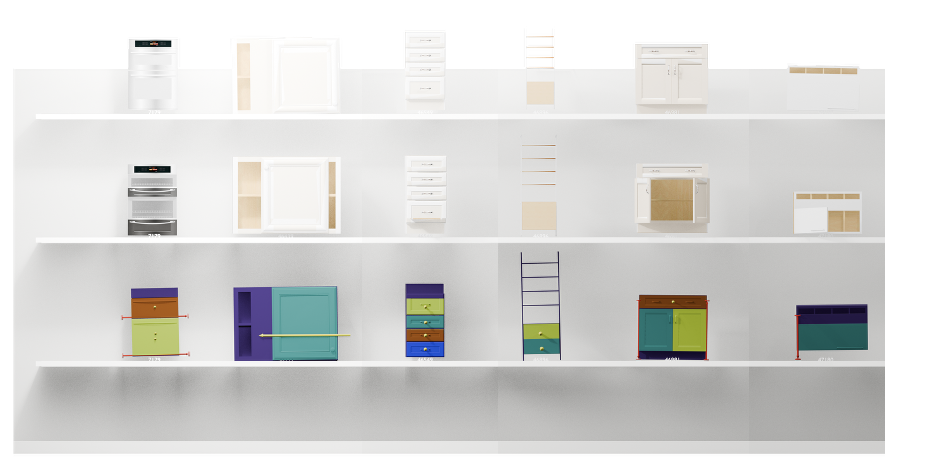
\includegraphics[width=0.8\textwidth]{figs/teaser_overview.png}
    \caption{\textbf{\method} directly infers the underlying articulated structure of an object from two distinct states,
    performing the state-of-the-art in terms of both accuracy and generalization.} 
    \label{fig:my_image} 
\end{figure}


\begin{abstract}

We present \method,
a feed-forward model that directly predicts all articulations of an object,
including part segmentation, kinematic structure, motion type, and continuous joint parameters,
from two distinct states of the same object.
Unlike existing \emph{single}-state feed-forward methods,
\method exploits the observed state change as direct evidence of articulation,
by learning to match the corresponding motion across the \emph{two} states,
rather than relying heavily on category-level priors learned from limited articulated-object annotations.
\method is a Siamese motion-based articulation transformer,
along with a cycle-consistency training objective that encourages consistent predictions under reversed state order.
We demonstrate the importance of the two-state formulation and cycle-consistency training for learning feed-forward articulations through extensive experiments.
We also show that \method achieves state-of-the-art performance on articulated structure recovery, with better generalization to novel object categories and more complex kinematic layouts.
% Additionally, we show that, with the help of VLMs, even a single state input can be extended to multiple states as conditioning for our model, further improving its performance and generalization.

% Recovering articulated 3D objects requires understanding not only their geometry, but also how their parts move and constrain one another.
% Existing feed-forward methods usually infer this structure from a single static observation, forcing the model to rely heavily on category-level priors learned from limited articulated-object annotations.
% We instead study articulation inference from two distinct states of the same object, where the observed state change directly exposes the moving parts and their underlying kinematics.
% We introduce \method, a feed-forward framework that takes two unorganized point clouds as input and predicts part segmentation, kinematic structure, motion type, and continuous joint parameters.
% \method uses a Siamese motion-based articulation transformer with shared part queries, query-to-point masked attention, point-to-query attention, and a cycle-consistency objective that encourages consistent predictions under reversed state order.
% This design allows the model to exploit cross-state geometric evidence without requiring point correspondences between the two observations, while retaining fast single-pass inference at test time.
% Experiments on articulated object benchmarks show that the two-state formulation substantially improves over single-state prediction and achieves state-of-the-art performance on articulated structure recovery, with ablations validating the contribution of cross-state reasoning and consistency training.
\end{abstract}

\section{Introduction}%
\label{sec:intro}

How do we perceive the articulated structure of an object?
Consider a child playing with an Optimus Prime robot~\footnote{Modern Transformer toys can contain more than 30 servomotors, with more than 100 moving parts.}.
Even without knowing its mechanism in advance, the child can quickly infer which parts move together, which joints rotate, and how one configuration transforms into another.
This ability does \emph{not} come from treating objects as static collections of isolated elements, but from observing the object across different states and reasoning about the \emph{motion} between them.

In this paper, we thus consider the problem of inferring the articulated structure of an object from \emph{two distinct states} of the same object,
rather than guessing it from a \emph{single static} observation.
Solving this task is particularly important for enabling AI systems to understand and interact with functional objects in our daily lives, such as drawers, laptops, and glasses, with broad applications in robotics~\cite{xiang2020sapien,li2024behavior}, virtual reality~\cite{chen2025freeart3d}, and embodied AI~\cite{Puig2023habitat,liigibson}.

Recently, several learning-based methods have been proposed to learn a feed-forward model that can directly infer part geometry and kinematics from visual inputs, such as a single image~\cite{chen2024urdformer,chen2025ArtiLatent} or a single 3D asset~\cite{che2024op,Goyal_2025_ICCV,li2025particulate}.
However, these methods still generalize poorly to unseen categories,
partly because they operate in a \emph{single-state} regime that learns the \emph{category-specific} kinematic priors from annotated training data.
However, current datasets with dense articulated annotations are extremely limited in scale and diversity~\footnote{Particulate~\cite{li2025particulate} combines PartNet-Mobility~\cite{Mo_2019_CVPR} and GRScenes~\cite{wang2024grutopia},
but still yields only 3,800 objects across 50 categories, most of which are furniture.}.
In stark contrast, the \emph{two-state} observation of the same object directly reveals the underlying motion and its articulation,
which is far easier to obtain at scale than dense kinematic annotations:
they can be collected from internet videos,
recorded through simple manual interactions~\cite{huang2026react3d},
or synthesized by modern multimodal foundation models,
like Seedance 2.0~\cite{seedance2026seedance}, Nano Banana Pro~\cite{gemini_image_pro}, and ChatGPT image 2.0~\cite{chatgpt_images_2_0}.

Drawing inspiration from this observation, we introduce \method, a novel paradigm that infers an object's articulation from two \emph{motion} states in a feed-forward manner.
With this \emph{two-state} learning paradigm, the task is formulated as learning to perform \emph{corresponding motion part matching} between the two states to identify the articulated parts with underlying motion and infer the kinematic structure, unlike the previous data-driven \emph{one-state} learning paradigm~\cite{che2024op,Goyal_2025_ICCV,li2025particulate} that learns the kinematic priors from annotated training data.
Such a formulation is more intuitive and reduces the task's learning difficulty,
enabling our model to achieve state-of-the-art performance and strong cross-dataset generalization ability on unseen categories.

In principle, several recent optimization-based methods~\cite{liu2023paris,chen2025freeart3d,ai2026aim} also exploit multi-state geometry to infer articulation (details shown in~\Cref{tab:related_articulation}), but they typically require test-time optimization and are therefore expensive and difficult to deploy.
In contrast, \method infers the full articulations in a single forward pass, in seconds, including part segmentation, kinematic hierarchy, motion type, and motion range.
Architecturally, it is a Siamese query-based transformer that takes two states as input and performs bidirectional information exchange between the two branches to capture the motion transformation.
To further align the model with physical laws, we introduce a cycle-consistency loss that enforces the model to produce consistent predictions when the order of the two states is swapped.

To summarize, we make the following contributions:
(1) We introduce \method, a novel feed-forward paradigm that learns to infer the full articulated structure of an object from \emph{two-state} observations.
(2) We demonstrate that the two-state design allows the model to easily predict articulated structure with state-of-the-art performance on both in-domain and out-of-domain benchmarks, and we strengthen this effect with a Siamese cycle-consistency training framework and objective.
(3) We also show that the additional state can be obtained cheaply in practice, like casual users' recorded media or current powerful multimodal foundation models generated images, making \method usable in real-world applications.

% \hrule

% \ruijie{
% In practice, we assume two input states of the same object, as our experiments show that this simple modification substantially improves cross-scene generalization while avoiding the need for complex multi-view inputs. More importantly, we found that the second state can be readily obtained by existing powerful multimodal foundation models ChatGPT image 2.0, making our approach both scalable and practical.


% Furthermore, unlike~\cite{li2025particulate} that predicts articulation from a single state, our method learns articulation in a way that aligns with physical laws, as it captures the underlying motion between two states rather than the instance category. 
% To verify this claim, we consider a dual problem: if we swap the order of the observed states, will the model still produce correct and consistent articulation predictions? Further experiments confirm this phenomenon. \todo{confirm this via cycle exp.} To further enhance this consistency, we design a Siamese framework that uses the reverse order of observed states to construct a cycle-consistency loss. Thanks to this training paradigm, our final model generates accurate, consistent articulated objects from arbitrary state changes, achieving a new state-of-the-art on both in-domain and out-of-domain benchmarks.

% To summarize, our key contributions are: (1) We introduce \method, a feed-forward method that utilizes two-state observations instead of one to generate articulated objects. Plus, we verify that the additional observation can be easily obtained by current VLMs. (2) We prove that the two-state design makes the model learn physical laws from articulated motion. A Siamese framework with a cycle-consistency constraint is also introduced to further confirm this. (3) Extensive experiments demonstrate that \method outperforms the state-of-the-art methods on both PartNet-Mobility and Lightwheel datasets. 
% }

% To effectively capture the geometric transformation between the two states, we build a dual-branch transformer backbone with a novel \emph{bidirectional Global Flow} mechanism.
% Specifically, the dual-branch transformer processes the two states in parallel,
% while the bidirectional Global Flow explicitly enforces information exchange between the two branches via cross-attention on part-centric queries from both states.
% With our dual-branch architecture and bidirectional Global Flow, the problem is formulated as to perform \emph{corresponding matching} between the two states to identify the moving parts and infer the kinematic structure, unlike the data-driven learning paradigm that relies on learning the kinematic priors from annotated training data~\cite{che2024op,Goyal_2025_ICCV,li2025particulate}.
% Such a formulation is more intuitive and reduces the task's learning difficulty,
% enabling our model to achieve state-of-the-art performance and strong generalization ability on unseen categories and real-world settings.

% Additionally, we also employ multiple decoders as previous works~\cite{Goyal_2025_ICCV,li2025particulate} that predict all the necessary parameters for a simulation-ready digital replica of the articulated object,
% including \emph{articulated} 3D part segmentation, kinematic hierarchy, motion type, and precise motion ranges.
% However, our model adopts a dual-branch architecture that processes the two states in parallel,
% and the decoders are designed to leverage the features from both branches to predict the parameters,
% rather than relying on a single branch that processes one state as previous works~\cite{Goyal_2025_ICCV,li2025particulate}.
% Although our inputs correspond to different states,
% they are derived from the identical object, and therefore should be consistent  the predicted parameters,
% such as part segmentation, kinematic hierarchy, and motion type (while the motion ranges are expected to be inversed).
% We thus introduce additional losses to explicitly enforce the consistency between the two branches,
% which further improves the performance and generalisation ability of our model.
% \todo{needs to refine depends on the final design.}
% Note that,
% since the state information flows bidirectionally through the attention, 
% our model does \emph{not} rely on any explicit correspondent points between the two states.

% On the in-domain PartNet-Mobility dataset~\cite{Mo_2019_CVPR}, our model achieves state-of-the-art performance on all the metrics, outperforming the previous best method by a large margin.
% More importantly, our model also demonstrates strong generalization ability on out-of-domain datasets, such as the real-world dataset LightWheel~\cite{li2025particulate}, without any fine-tuning, which is a significant improvement over previous methods that fail to generalize to unseen categories and real-world settings. \todo{refine based on the final results}
% Furthermore,
% extensive ablation studies and analysis underscore the significance of our two distinct states formulation,
% along with the dual-branch architecture and bidirectional Global Flow mechanism, in effectively capturing the geometric transformation and inferring the articulated structure of objects. 


% Articulated objects, ranging from common household items like drawers and laptops to complex industrial machinery, are ubiquitous in our daily environments and central to human-scene interactions. Consequently, the perception and understanding of these objects are critical across domains such as virtual and augmented reality (VR/AR), industrial design, and computer animation. More importantly, constructing accurate digital replicas of articulated objects is a foundational requirement for robotics and embodied AI, enabling agents to simulate and interact with the physical world effectively.

% Although recent advancements in 3D generation and reconstruction have significantly automated the creation of static assets, modelling articulated objects remains a formidable challenge. Unlike static geometries, articulated objects consist of interconnected parts that exhibit constrained motion. Recovering their digital replicas requires not only high-fidelity geometric reconstruction but also the precise inference of the underlying kinematic structure and functional mechanisms.

% In this paper, we observe the essence of articulation: the relative motion between parts can be effectively captured by observing just two distinct configurations. We introduce a novel framework that infers articulated structure from two states by leveraging the geometric transformation between a canonical state and an articulated state.

% To achieve this, we propose \emph{TWIST}, an end-to-end neural architecture that jointly processes two point-cloud states to extract a comprehensive kinematic graph. At the core of our method is a dual-branch transformer backbone equipped with a novel bidirectional Global Flow mechanism. By explicitly enforcing cross-attention between object-centric queries from the two states (q0 and q1), our network inherently learns the temporal and spatial correspondences necessary to identify moving parts without relying on explicit point-level tracking.

% Furthermore, decomposing an object into functional parts is often ambiguous. To address this, our architecture incorporates a Multi-Hypothesis Mask Decoder, allowing the network to propose multiple valid part segmentation configurations and select the most geometrically consistent one.

% Beyond mere segmentation, our framework fully parameterises the articulation. By pooling features based on the predicted part assignments, our motion and hierarchy decoders predict the pairwise adjacency matrix (the kinematic structure) and classify the motion type (e.g., revolute, prismatic). For precise physical simulation, we regress exact motion parameters, utilising Plücker coordinates to robustly represent 3D motion axes and predicting the continuous ranges of motion for each joint.

% In summary, our main contributions are as follows: 

% \textbf{A Dual-State Formulation:} We introduce a novel approach to articulated object understanding that bypasses the need for dense video sequences, successfully inferring complex kinematics from just two distinct structural states.

% \textbf{Bidirectional Global Flow Architecture:} We propose a dual-branch transformer equipped with inter-branch cross-attention, enabling effective feature exchange and implicit motion tracking between states.

% \textbf{Comprehensive Kinematic Parameterisation :} Our end-to-end framework jointly predicts multi-hypothesis part segmentations, kinematic hierarchies, motion types, and precise joint parameters (axes and ranges), generating a complete, simulation-ready digital replica.
% \label{sec:intro}
\section{Related Work}%

% \ruijie{
As summarized in Table~\ref{tab:related_articulation}, we divide existing articulated reconstruction approaches into three types: optimization-based, learning-based, and generation-based methods.

\paragraph{Optimization-based articulated reconstruction.} 
An important line of work studies articulated objects through per-instance reconstruction from multiple observations. Early methods~\cite{liu2023paris,tseng2022cla,wei2022self} recover geometry and articulation by fitting a deformable NeRF~\cite{mildenhall2020nerf} to a specific object observed across multiple views or articulation states. More recent dynamic reconstruction methods~\cite{liu2025artgs,wu2025reartgs,ai2026aim,shen2025gaussianart,liu2025videoartgs,guo2026articulat3d} further exploit motion videos or continuous interaction to disentangle moving parts via Gaussian Splatting~\cite{kerbl20233d}. However, they are still optimization-intensive pipelines whose quality depends on how well the observations cover the scene.
Therefore, a generalizable end-to-end articulation estimation is what physical-world modeling really needs: not only for fast inference but also for a full understanding of physical cues.

\paragraph{Learning-based articulated reconstruction.} 
Recent learning-based methods usually predict articulated structure from a single image~\cite{chen2024urdformer,li2026monoart} or a single 3D observation~\cite{che2024op,Goyal_2025_ICCV,li2025particulate,gao2025meshart,song2025magicarticulate,li2025urdfanything}. 
For example, Particulate~\cite{li2025particulate} takes a single point cloud as input, and outputs the part segmentation of the point cloud and the kinematic parameter of those parts. 
Compared with per-instance optimization, these feed-forward methods are much more scalable and can perform inference directly and quickly. 
However, these methods also have limitations.
Although they curate diverse articulation datasets for training, their generalization remains unsatisfactory, even within the same category. 
% This limitation becomes more severe in open-world settings, where object geometry and kinematic layouts can differ substantially from those seen during training. 
We argue that this is because they use only a single static state as conditioning for predicting action-based articulation, which makes the task itself ambiguous: a single observation may correspond to different articulation patterns, even within the same category.
Therefore, we propose using multi-state observations as conditioning and designing an action-wise framework to resolve the ambiguity. 
% Furthermore, we prove that, with the help of VLMs, even a single state input can be extended to multiple states as conditioning for our model, outperforming state-of-the-art methods in a fair comparison.

\paragraph{Generation-based articulated reconstruction.} 
Another direction focuses on constructing articulated assets by retrieval, composition, or generation rather than directly inferring articulation from visual observations. 
These methods~\cite{liusingapo,lei2023nap,liu2024cage,chen2025freeart3d,chen2025ArtiLatent,wu2026urdfanything_plus,Su_2025_CVPR} assemble reusable parts, invoke articulation-aware priors, or combine generation with structural reasoning to produce simulation-ready articulated assets. 
For example, URDF-Anything+ takes an image and a mesh as inputs and leverages DiT~\cite{peebles2023scalable,chen2025autopartgen} to autoregressively generate articulated objects.
Recent multimodal frameworks~\cite{wang2025kinematify,qiu2025articulate,lu2025dreamart,wu2025dipo} further advance articulated asset generation using generative priors from VLMs~\cite{hurst2024gpt,gemini_image_pro}. 
Despite their impressive generalization in open-world scenes, they suffer from slow inference, LLM illusions, and difficulty handling complex topology.
% }



% \paragraph{Reasoning from observed state change.} Our work is motivated by the observation that articulation is most reliably revealed by how an object changes across states. Prior methods have leveraged multiple observations mainly in optimization-heavy reconstruction pipelines~\cite{liu2023paris,tseng2022cla,wei2022self}, where motion evidence is absorbed through iterative fitting rather than encoded by a generalizable feed-forward predictor. In contrast, we study articulation inference from two observed 3D states of the same object within a single forward pass. This setting lies between single-state prediction and full reconstruction: it preserves factual motion evidence from state change while avoiding per-instance test-time optimization. More importantly, our method does not merely treat the second state as additional input. Instead, it uses shared part queries to explain both states with a common part ordering, and refines query-to-point reasoning through mask-guided attention feedback. The shared queries establish cross-state part correspondence, while the mask-guided refinement localizes moving parts in each state before kinematic decoding. This distinction separates our method from single-state feed-forward baselines, generic mask-based part segmentation methods, and optimization-based reconstruction pipelines, and underlies the stronger robustness and cross-scene generalization observed in our experiments.


\label{sec:related}

\begin{figure}[t]
    \centering
    % 第一张图及其标题
    \begin{minipage}[b]{0.32\linewidth}
        \centering
        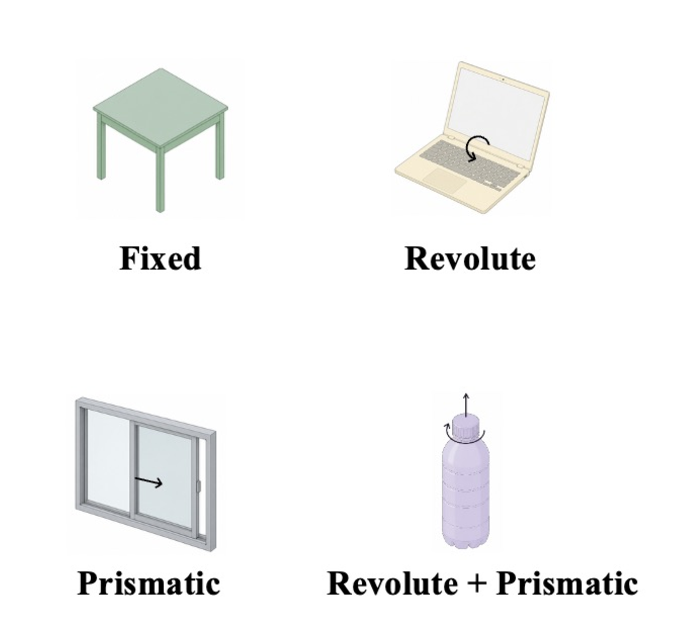
\includegraphics[width=\linewidth]{figs/3_ART_type.pdf}
        \caption{Articulation types.} % 独立的标题 1
        \label{fig:art_type}
    \end{minipage}
    \hfill % 撑开中间间距
    % 第二张图及其标题
    \begin{minipage}[b]{0.65\linewidth}
        \centering
        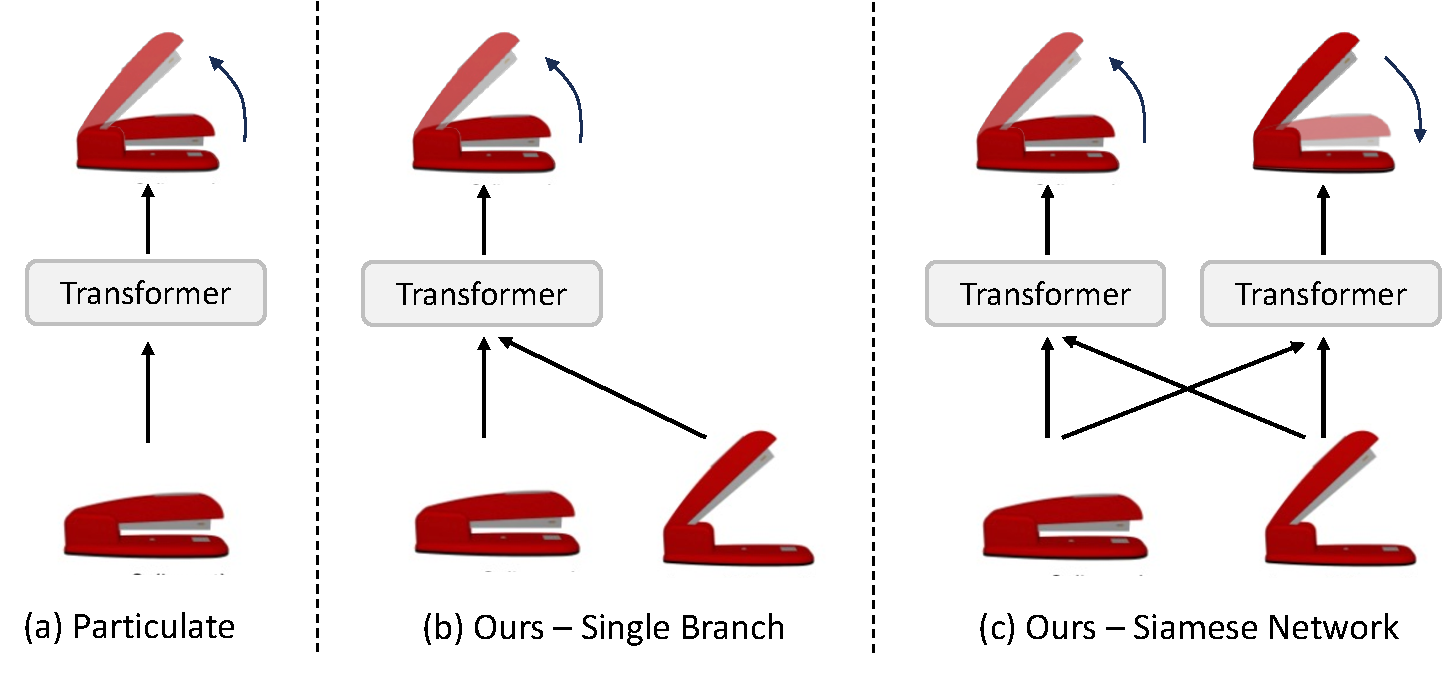
\includegraphics[width=\linewidth]{figs/5_model_diff.pdf}
        \caption{The different pipelines.} % 独立的标题 2
        \label{fig:model_diff}
    \end{minipage}
\end{figure}


\section{Method}%
\label{sec:method}

We introduce \method,
a Siamese transformer architecture for learning part segmentation and articulation parameters from two states ($s_0$ and $s_1$) of an articulated object.
We first formulate the problem setting in~\Cref{sec:problem},
followed by our Siamese transformer architecture in~\Cref{sec:backbone} and its multi-task decoder in~\Cref{sec:decoder}.
Finally, we describe the training objectives in~\Cref{sec:training}.

\begin{figure}[t]
    \centering
    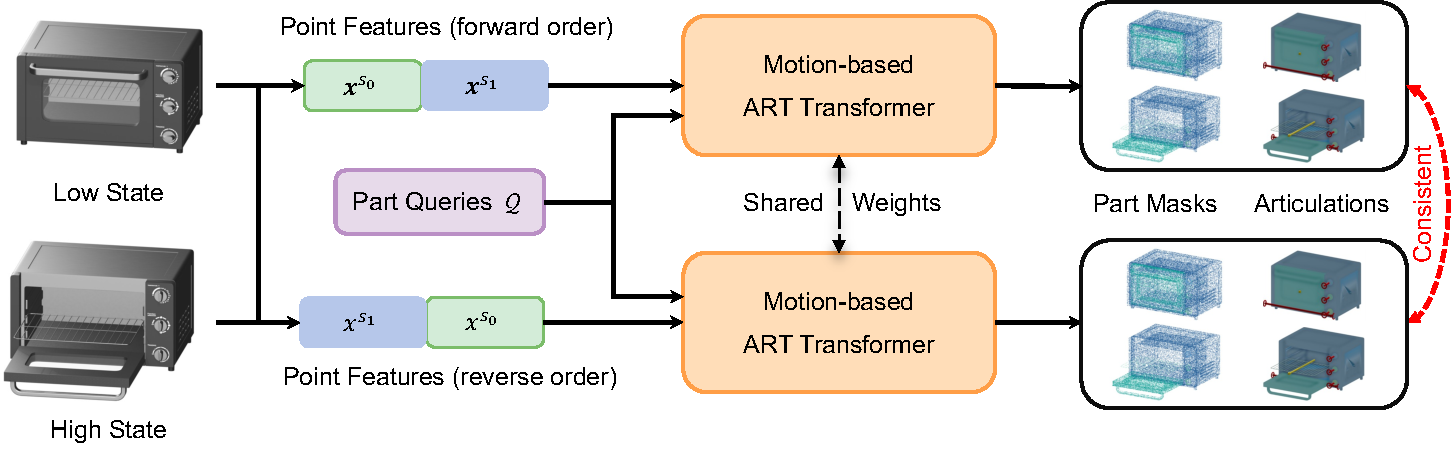
\includegraphics[width=\linewidth]{figs/framework.pdf}
    \caption{\textbf{Overview of \emph{\method}.} Given two observed states of the same object, our framework jointly reasons over cross-state geometry to predict part segmentation and the underlying kinematic structure. We use a set of shared queries to aggregate two-state features, with each query representing a rigid part. The overall Siamese framework consists of two branches: forward order and reverse order. Each branch predicts both part segmentation of two states and articulation parameters.}
    \label{fig:method_overview}
\end{figure}

% \ruijie{
\subsection{Problem Formulation}
\label{sec:problem}
The input is two distinct physical states of an object,
representing the articulation motion from start $s_0$ to end $s_1$.
Specifically, the observations are two unorganized point clouds 
$\{\mathcal{P}^{(s_i)}\}_{i=\{0,1\}}$,
where each
$\mathcal{P}^{(*)} = \{\bm{p}_i^{(*)}\in\mathbb{R}^3\}_{i=1}^N$
is sampled from two states of the object mesh
$\{\mathcal{M}^{(s_i)}\}_{i=\{0,1\}}$,
respectively,
where $N$ is the number of sampled points.
Our goal is to learn a Model
$f_{\bm{\theta}}$
that maps these two states of point clouds to a set of part segmentation masks and articulation parameters:
\begin{equation}
    \label{eq:goal}
    f_{\bm{\theta}} : \{\mathcal{P}^{(s_i)}, \mathcal{N}^{(s_i)}, \bm{F}^{(s_i)}\}_{i=\{0,1\}} \mapsto \{M^{(s_i)}, \mathcal{G}^{(s_i)}, \Theta^{(s_i)}\}_{i=\{0,1\}},
\end{equation}
where $\mathcal{N}^{(s_i)}$ and $\bm{F}^{(s_i)}$ are the surface normal and part features from off-the-shelf extractors of the point cloud from state $s_i$, respectively.

We predict all outputs for both states.
However, to simplify the notation, we will only describe the output of one state, while the other state follows the same procedure.
We predict the segmentation masks $M \in \{0,1\}^{N \times K}$ for $K$ \emph{kinematic parts}
and infer the underlying \emph{kinematic graph}
$\mathcal{G} = \{\mathcal{V}, \mathcal{E}\}$,
where
node $\mathcal{V}$ composed by $K$ kinematic parts and
edge $\mathcal{E}$ is a directed \emph{kinematic tree}
$J_{K \times K}$
that defines the joint connectivity between parts.
We also predict the \emph{articulation parameters} of joints $\Theta=\{\mathcal{A}, \mathcal{R}, \mathcal{T}\}$,
where
$\mathcal{A}$ denotes the articulation types,
which are predefined as four types:
$\{$fixed, \emph{revolute}, \emph{prismatic}, and \emph{revolute + prismatic}$\}$, as shown in~\Cref{fig:art_type};
$\mathcal{R} = \{(\bm{\omega}_e, \bm{q}_e, \alpha_e)\}_{e \in \mathcal{E}}$ denotes the revolute parameters, where $\bm{\omega}_e \in \mathbb{S}^2$ is a unit rotation-axis direction, $\bm{q}_e \in \mathbb{R}^3$ is a pivot point on that axis, and $\alpha_e \in \mathbb{R}$ is the range
$(\alpha_{\min}, \alpha_{\max})$
of the rotation angle between two states;
and $\mathcal{T} = \{(\bm{d}_e, l_e)\}_{e \in \mathcal{E}}$ denotes the prismatic parameters,
where $\bm{d}_e \in \mathbb{S}^2$ is a unit translation direction and $l_e \in \mathbb{R}$ is the range
$(l_{\min}, l_{\max})$
of the translation distance between two states.

\heading{\emph{Multi}-state \vs \emph{single}-state}
We implement the model
$f_{\bm{\theta}}$
as a feed-forward Siamese transformer architecture
with shared weights,
and $\bm{\theta}$ are the learnable parameters.
Prior feed-forward methods~\cite{chen2024urdformer,chen2025ArtiLatent,che2024op,Goyal_2025_ICCV,li2025particulate} usually optimize $\bm{\theta}$ with a single state as input.
This is partly reliable if the training data is sufficiently large and diverse in the deep learning era, but it is \emph{not} the case in practice, especially for kinematic annotated 3D.
We instead consider a new \emph{feed-forward} paradigm that uses \emph{two-state} of an object as input to learn the underlying physical rules of articulation from the state motion change,
which is more efficient and generalizable than learning priors from a single state.
The \emph{core insight} is that the two states of the same object directly reveal the articulation attributes,
while two-state observations are also easily obtained in real-world applications, \eg, by scanning or capturing an object before and after interaction.
Notably, we do \emph{not} assume any point correspondence between two states,
which is more challenging but also more practical in real-world applications.
We select \emph{two}-state because it is the minimum number of states that can reveal the articulation attributes,
but our design is \emph{not} specific to two states and can be easily extended to more states if needed.

% \subsection{Overall Framework}
% As shown in~\Cref{fig:method_overview}, our method, \method, addresses this problem with a Siamese transformer framework. 
% First, we extract features from two point clouds, $P_0$ and $P_1$, and concatenate the resulting feature sets to serve as context information, in ascending and descending order, respectively. 
% A set of part queries is then initialized to perform cross-attention on the context features in each branch.
% The updated part queries are finally passed through the ART Decoder to predict the part segmentation and articulation parameters.
% We use ground-truth annotations for segmentation and articulation supervision and design a consistency loss to further enforce symmetry between the two dual branches.
% The overall framework offers two-sided advantages:
% (1) efficient learning, since the Siamese network is trained on two dual samples in each iteration;
% (2) fast inference speed, since we only need a single branch for inference.
% }
% The two states are processed as separate point streams, but they are interpreted by a single set of part queries that is reused across both states. 
% This design ensures that each query represents the same semantic and kinematic part before and after motion, thereby avoiding the need to solve an additional query-matching problem across states. 
% The resulting part queries are used by a Mask2Former-style mask refinement decoder and by kinematic heads that predict part connectivity, motion type, and joint parameters.

\subsection{Two-state Motion-based Articulation Transformer}
\label{sec:backbone}

At a high level, \method is a Siamese transformer architecture with shared weights that takes two states of point clouds as input,
and learn the underlying physical rules of articulation from the state motion change,
rather than learning articulation priors from a single state as in prior feed-forward methods~\cite{li2025particulate,li2025urdfanything,wu2026urdfanything_plus}.
The key insight of our design is that we can simultaneously infer full articulation attributes for two states,
using only one set of shared part queries,
and achieve more robust, generalizable performance by enforcing cycle consistency between them.

However, this architecture design is non-trivial because: 
(1) The two states of point clouds are randomly sampled and unorganized, \ie, there are no matching points between the two states. 
\footnote{Note that we deliberately did not perform consistent sampling of the point clouds to generate data samples, because it is too difficult to obtain the matching points in the second state as input in practical applications.}
(2) The motion of articulated parts makes the point correspondence more complex, \ie, those points of the moving parts are not even spatially aligned.
The missing point correspondence indicates that although the additional state provides richer articulation cues, the network still requires careful design to fully utilize them.
To address this issue, we develop a dedicated two-state Motion-based Articulation Transformer with a Siamese architecture.

\heading{Siamese Architecture with Shared Part Queries}
As shown in~\Cref{fig:model_diff} (a),
prior feed-forward methods predict full articulation parameters by learning from a single state of an object.
However, our model includes two states of an object as input.
We could instead train the network by directly concatenating the two states with $2N$ points
as input and predicting the full articulation attributes for both states at the same time (\Cref{fig:model_diff} (b)). 
While this na\"ively concatenation works by learning with two states,
it does not explicitly enforce the part queries to learn the same semantic and kinematic part across two states.
More importantly,
since we argue the \emph{two-state} learning paradigm learns articulation in a way that aligns with physical laws, as it captures the underlying motion between two states rather than the instance category.
Hence, if we swap the order of the observed states, the model should still produce correct and consistent predictions.
We achieve this by designing a Siamese architecture with shared weights and part queries (\Cref{fig:model_diff} (c)).
Enforcing consistency between two branches using the cycle consistency loss yields more robust and generalizable performance, as shown in our experiments.
% \heading{Masked Query-to-point Attention} \cxz{remove it as it does not mean a lot from the ablations}
Our transformer architecture is inspired by Particulate~\cite{li2025particulate},
but features several key differences that allow us to train with two states and ensure the consistency between the two branches.

For each \textbf{input} point
$\bm{p}_i\in\mathcal{P}$,
we still concatenate its coordinates, normals, and part features in the channel dimension to obtain the input point features
$\bm{x}_i = \big[\,\bm{p}_i, \bm{n}_i, \bm{f}_i\,\big] \in \mathbb{R}^{3 + 3 + d}$.
But now we have two states of points that are concatenated in the token dimension, \ie, $\{\bm{x}_i\}_{i=1}^{2N}$.
In our final reverse-order modal (\Cref{fig:method_overview} (c)),
we simply swap the order of two states of input point features.

For the \textbf{part queries},
we still use a set of shared learnable queries $\mathcal{Q} \in \mathbb{R}^{K_{\max} \times D}$,
where $K_{\max}$ is set to be particularly large to cover the maximum number of parts in the training data,
as the actual number of parts is unknown a priori,
and $D$ is the query dimension.

The \textbf{attention blocks} 
is a sequence of self-attention on part queries, followed by query-to-point attention and point-to-query attention.
Here, we apply the masked attention mechanism~\cite{cheng2022masked} to the query-to-point attention,
which first predicts a binary mask for each query to indicate the activated points,
and then uses the predicted mask to modulate the attention weights in the next layer of attention.
The detailed description is provided in~\Cref{sec:supp_impl_compute_impact}.
This masked attention mechanism is crucial for our model to learn from two states without point correspondence,
as it forces the part queries to focus on the activated areas of the same part across two states.
After several layers of attention, we obtain the updated part queries
$\tilde{\mathcal{Q}} \in \mathbb{R}^{K_{\max} \times D}$,
and point tokens $\tilde{\mathcal{P}} \in \mathbb{R}^{2N \times D}$.

\subsection{Prediction Heads}
\label{sec:decoder}
Following Particulate~\cite{li2025particulate}, we use several MLPs to predict the part segmentation
$M$,
the kinematic graph $\mathcal{G}$,
and the articulation parameters $\Theta$.
Note that we primarily describe the decoding process for the forward-order branch, while the other branch follows a similar procedure.

We use an MLP to predict the \textbf{point segmentation mask}
$\hat{M} = \operatorname{MLP} (\tilde{\mathcal{Q}}, \tilde{\mathcal{P}})$,
where $\hat{M}\in \mathbb{R}^{2N \times K_{\max}}$,
which indicates the probability of part segmentation for each point.
Note that it contains points from both states,
even in one branch.

We predict the \textbf{kinematic graph} $\hat{\mathcal{G}}$,
which is represented as a kinematic tree $\hat{J} \in \{0,1\}^{K_{\max} \times K_{\max}}$,
by applying an MLP to every ordered query pair
$\hat{J}_{ij} = \operatorname{MLP} (\tilde{Q}_i,\tilde{Q}_j)$,
where $\tilde{Q}_i,\tilde{Q}_j$ correspond to the corresponding query of part $i$ and $j$, respectively.
Following the URDF definition, we designate one basic part as the root node of the kinematic tree and restrict each part to have at most one parent node.
Therefore, given actual $K$ parts, there are exactly $K-1$ joints,
where $K \le K_{\max}$.

We use several MLPs to predict the \textbf{articulation parameters} $\hat{\Theta} =\operatorname{MLPs} (\tilde{\mathcal{Q}})$,
where $\hat{\Theta} = \{\hat{\mathcal{A}}, \hat{\mathcal{R}}, \hat{\mathcal{T}}\}$.
Note that,
separate MLPs are used to predict different types of parameters in $\hat{\Theta}$.
As mentioned in~\Cref{sec:problem},
we predefine four types of articulation.
The articulation type $\hat{\mathcal{A}}$ is predicted by a classification MLP to output the logits of query part $i$ belonging to each of the \emph{four} types.
The revolute parameters $\hat{\mathcal{R}} = \{\hat{\bm{\omega}}_e, \hat{\bm{q}}_e, \hat{\alpha}_e\}_{e\in\mathcal{E}}$
and prismatic parameters $\hat{\mathcal{T}} = \{\hat{\bm{d}}_e, \hat{\bm{q}}_e\}_{e\in\mathcal{E}}$ are predicted by regression MLPs for each joint $e$.
Note that the predicted parameters of a joint are only valid if the corresponding part is classified as a moving part, \ie, revolute, prismatic, or revolute + prismatic.

% Our predication heads are mainly built on Particulate~\cite{li2025particulate},
% which is not our main contribution.
% For more details of the architecture design and implementation, please refer to~\cite{li2025particulate}.

\subsection{Training}
\label{sec:training}

During training, we sample two point cloud states and their corresponding ground-truth annotations.
Note that,
while we have different states,
the kinematic tree, articulation type, and joint parameters should be the same for both states.
We only swap the part segmentation masks between the two states, and also flip the ranges of revolute and prismatic motion to align the motion directions.
This design enforces the model to learn the same kinematic structure and motion attributes across two states.

% We train \method end-to-end. For each training sample, we extract its two-state point cloud as input and have the siamese network predict, for each branch, the part segmentation $M$, the kinematic tree $J$, and the articulation parameters $\theta = \{A, R, T\}$.
% Meanwhile, the corresponding ground truth annotations are curated to provide direct supervision.
% However, the predicted class-agnostic parts do not correspond to the ground truth on a one-to-one basis; we still need a matching procedure for backpropagation. 

\heading{Part Matching with Ground Truth}
We use the Hungarian Matching to build part correspondence following~\cite{li2025particulate,carion2020end}. The difference with~\cite{li2025particulate} is that since we have two sets of output queries that predict two-state part segmentation, we only perform Hungarian Matching for the rest state and enforce the articulated state following the same matching orders. 
In this way, we ensure that the two output queries predict consistent part segmentation.

\heading{Training Losses}
We train the \method end-to-end using a multi-task loss:
\begin{equation}
    \label{eq:total_loss}
    \mathcal{L} = \underbrace{\mathcal{L}_\text{seg}^\text{f}+\mathcal{L}_\text{art}^\text{f}}_\text{forward branch loss} + \underbrace{\mathcal{L}_\text{seg}^\text{r}+\mathcal{L}_\text{art}^\text{r}}_\text{reverse branch loss} +  \underbrace{\lambda_\text{cycle} \mathcal{L}_\text{cycle}}_\text{cycle loss},
\end{equation}
where $\mathcal{L}^{*}_\text{seg}=\sum_{i=\{0,1\}}\operatorname{CE}(\hat{M}^{(s_i)}, M^{(s_i)})$ is the cross entropy loss for \textbf{part segmentation} for both states
$s_i$ in branch $*$,
$\mathcal{L}^{*}_\text{art} = \operatorname{BCE}(\hat{\mathcal{J}},\mathcal{J}) + \operatorname{CE}(\hat{\mathcal{A}},\mathcal{A}) + \ell_1(\hat{\mathcal{R}}, \mathcal{R}) + \ell_1(\hat{\mathcal{T}}, \mathcal{T})$
is the \textbf{articulation loss} for branch $*$,
which includes binary cross-entropy loss for the kinematic tree $\mathcal{J}$, cross-entropy loss for the articulation type $\mathcal{A}$, and L1 losses for the revolute parameters $\mathcal{R}$ and prismatic parameters $\mathcal{T}$.
The motion ranges of revolute and prismatic joints in the two branches are flipped.
To simplify the notation,
we just use $\mathcal{R}$ and $\mathcal{T}$ to represent them.
More details are provided in~\Cref{sec:supp_loss_details}.

Since the two branches solve dual problems,
we can naturally construct \textbf{cycle consistency loss}
$\mathcal{L}_{cycle}$ between the branches,
which includes both the part segmentation loss and the articulation loss:
\begin{equation}
    \mathcal{L}_\text{cycle} =
    \operatorname{BCE}(\hat{\mathcal{J}_f},\hat{\mathcal{J}_r}) + \operatorname{CE}(\hat{\mathcal{A}_f},\hat{\mathcal{A}_r}) + \ell_1(\hat{\mathcal{R}_f},\hat{\mathcal{R}_r}) + \ell_1(\hat{\mathcal{T}_f},\hat{\mathcal{T}_r})
    + \sum_{i=\{0,1\}}\operatorname{CE}(\hat{M}^{(s_i)}_f, \hat{M}^{(s_i)}_r)
\end{equation}
where the lower script $f$ and $r$ denote the forward-order branch and reverse-order branch, respectively.
This cycle consistency loss enforces that the two branches produce consistent predictions, leading to more robust and generalizable performance, as shown in our experiments.

% \hrule

% \ruijie{

% \paragraph{Cycle Consistency loss.}
% Since the two branches solve dual problems, we can naturally construct consistency constraints between the branches. Specifically, for the reverse-order branch, we swap the part segmentation predictions to match the parts and flip the ranges of revolute and prismatic motion to align the motion directions. The cycle consistency loss includes both the part segmentation loss and the articulation loss:
% \begin{equation}
%     \mathcal{L}_{cycle} = \sum_{i=\{0,1\}}\text{CE}(M_i, \widetilde{M}_{1-i}) + \sum \left ( \text{BCE}(J,\widetilde{J}) + \text{CE}(A,\widetilde{A}) + ||R+\widetilde{R}||_1 + ||T+\widetilde{T}||_1\right )
% \end{equation}
% where $\widetilde{M},\widetilde{J},\widetilde{A},\widetilde{R},\widetilde{T}$ are the prediction results of the reserve-order branch.
% }

% \paragraph{Total loss.}
% The final training loss is summarized as:
% \begin{equation}
%     \mathcal{L}_{total} = \underbrace{\mathcal{L}_{seg\_1}+\mathcal{L}_{art\_1}}_{branch~1~loss} + \underbrace{\mathcal{L}_{seg\_2}+\mathcal{L}_{art\_2}}_{branch~2~loss} +  \underbrace{\lambda_{cycle} \mathcal{L}_{cycle}}_{cycle~loss}
% \end{equation}
% }

% \method is trained with supervision on segmentation, kinematic structure, motion class, and continuous motion parameters. The segmentation objective combines pointwise cross-entropy and Dice loss over the concatenated two-state masks. The graph decoder is trained with binary cross-entropy over valid part pairs, and the motion classifier is trained with cross-entropy over valid parts. Continuous joint parameters are supervised with L1 losses on active revolute and prismatic joints, while inactive motion heads are ignored through valid-motion masks. For the closest-axis representation, we additionally supervise the predicted closest point on the revolute axis for points belonging to revolute parts. The final objective is a weighted sum of these terms:
% \begin{equation}
%     \mathcal{L} =
%     \lambda_{\mathrm{mask}}\mathcal{L}_{\mathrm{ce}} +
%     \lambda_{\mathrm{dice}}\mathcal{L}_{\mathrm{dice}} +
%     \lambda_{\mathrm{edge}}\mathcal{L}_{\mathrm{edge}} +
%     \lambda_{\mathrm{cls}}\mathcal{L}_{\mathrm{motion}} +
%     \lambda_{\mathrm{param}}\mathcal{L}_{\mathrm{param}} +
%     \lambda_{\mathrm{axis}}\mathcal{L}_{\mathrm{closest}}.
% \end{equation}
% This objective encourages the shared part queries to explain both observed states consistently while still preserving point-level evidence for precise mask and joint prediction.


\section{Experiments}%

\label{sec:experiments}

We evaluate the performance of \method in part segmentation and articulation estimation for both rest and articulated states.
Our experiments mainly answer three questions:
(1) whether two-state reasoning improves the model generalization over single-state reasoning;
(2) whether the network achieves consistent predictions between two states and whether the Siamese framework further improves the consistency;
and (3) whether the recovered articulation is good enough to be exported as a URDF asset for downstream robot simulation.
We first describe the evaluation protocol, then report comparisons with state-of-the-art methods, ablations, and an application in RoboTwin.

\begin{table}[t]
\centering
\small
\caption{
\textbf{Evaluation on rest and fully articulated states.}
For each dataset we report rest-pose segmentation (gIoU, part-wise Chamfer distance PC, and mIoU) and articulated geometry (gIoU, PC, and whole-object Chamfer distance OC).
All metrics are computed with penalties applied to unmatched parts.
--: method is not applicable for the articulated state.
1@10: best sample out of 10 predictions per instance.
Colors: \best{best} and \secondbest{second best}.
}%
\label{tab:combined-comparison}
\setlength{\tabcolsep}{3pt}
\renewcommand{\arraystretch}{1.1}
\resizebox{\linewidth}{!}{%
\begin{tabular}{@{}lcccccc ccccccc@{}}
\toprule
& \multicolumn{6}{c}{\textbf{Lightwheel}}
& \multicolumn{6}{c}{\textbf{PartNet-Mobility}} \\
\cmidrule(lr){2-7}\cmidrule(lr){8-13}
\textbf{Method} & \multicolumn{3}{c}{\textbf{Rest-Pose Seg.}}
& \multicolumn{3}{c}{\textbf{Articulated States}}
& \multicolumn{3}{c}{\textbf{Rest-Pose Seg.}}
& \multicolumn{3}{c}{\textbf{Articulated States}} \\
\cmidrule(lr){2-4}\cmidrule(lr){5-7}\cmidrule(lr){8-10}\cmidrule(lr){11-13}
& gIoU$\uparrow$ & PC$\downarrow$ & mIoU$\uparrow$
& gIoU$\uparrow$ & PC$\downarrow$ & OC$\downarrow$
& gIoU$\uparrow$ & PC$\downarrow$ & mIoU$\uparrow$
& gIoU$\uparrow$ & PC$\downarrow$ & OC$\downarrow$ \\
\midrule
% PartField~\cite{liu2025partfield}
%   & 0.079 & \best{0.106} & 0.264
%   & -- & -- & --
%   & 0.183 & 0.123 & 0.361
%   & -- & -- & -- \\
P3SAM~\cite{ma2025p3sam}
  & 0.122 & 0.177 & 0.411
  & -- & -- & --
  & -0.116 & 0.261 & 0.267
  & -- & -- & -- \\
\midrule
SINGAPO~\cite{liusingapo}
  & -0.097 & 0.234 & 0.273
  & -0.102 & 0.329 & 0.018
  & 0.262 & 0.124 & 0.468
  & 0.255 & 0.184 & 0.046 \\
SINGAPO~\cite{liusingapo} (1@10)
  & -0.050 & 0.221 & 0.297
  & -0.056 & 0.261 & 0.019
  & 0.271 & 0.117 & 0.471
  & 0.264 & 0.168 & 0.041 \\
Articulate AnyMesh~\cite{qiu2025articulate}
  & 0.172 & 0.190 & 0.452
  & 0.158 & 0.237 & 0.010
  & 0.383 & 0.104 & 0.542
  & 0.378 & 0.251 & 0.022 \\
Particulate~\cite{li2025particulate}
  & 0.332 & \secondbest{0.168} & 0.576
  & 0.305 & 0.208 & 0.009
  & {0.880} & \secondbest{0.003} & {0.884}
  & {0.843} &{0.022} & \secondbest{0.003} \\
\textbf{\method (Single)}
  & \secondbest{0.489} & \best{0.156} & \secondbest{0.578}
  & \secondbest{0.474} & \secondbest{0.194} & \best{0.003}
  & \secondbest{0.924} & \best{0.002} & \secondbest{0.936}
  & \secondbest{0.888} &\secondbest{0.007} & \best{0.001} \\
\textbf{\method (Siamese)}
  & \best{0.544} & \best{0.156} & \best{0.647}
  & \best{0.512} & \best{0.188} & \secondbest{0.005}
  & \best{0.931} & \secondbest{0.003} & \best{0.939}
  & \best{0.890} & \best{0.005} & \best{0.001} \\
\bottomrule
\end{tabular}%
}
\end{table}


\subsection{Experimental Setup}
\label{sec:exp_setup}

\heading{Training Datasets}
We train \method on the PartNet-Mobility~\cite{Mo_2019_CVPR} and GRScenes~\cite{wang2024grutopia} datasets.
For PartNet-Mobility, we follow the train-test split of SINGAPO~\cite{liusingapo}; for GRScenes, we use all articulated assets for training.
We set the maximum number of parts to $K_{\max}=16$ and discard objects with more than 16 articulated parts, yielding 3,800 training objects across 50 categories.

\heading{Testing Datasets}
For evaluation, we use the PartNet-Mobility test split, which contains 7 common articulated-object categories, and the Lightwheel benchmark~\cite{lightwheel_simready_2025}, which contains 243 high-quality articulated objects spanning 14 categories.
For every object, we sample two distinct physical states and convert them into a pair of unorganized point clouds.
Since the two point clouds are sampled independently, the model does not rely on explicit point correspondence between the states.


% \heading{Baselines.}
% We compare against representative methods for segmentation, retrieval-based reconstruction, and feed-forward articulation inference.
% The baselines include a naive part-matching baseline, SINGAPO~\cite{liusingapo}, PartField~\cite{liu2025partfield}, P3SAM~\cite{ma2025p3sam}, Articulate AnyMesh~\cite{qiu2025articulate}, and Particulate~\cite{li2025particulate}.
% For methods that can benefit from mesh connectivity, we report connectivity-assisted variants marked by $^\dagger$.
% This protocol separates the effect of geometric connectivity from the ability to infer articulation from the observed states.

\heading{Implementation details}
Each input state is represented by a point cloud sampled from the corresponding mesh.
Following Particulate~\cite{li2025particulate}, we augment point coordinates with surface normals and PartField features.
At test time, \method uses a single forward branch to predict the part masks, kinematic tree, motion type, joint axes, and motion ranges, \ie, the reverse-order branch and cycle-consistency objective are used only during training. Training the main model takes approximately three days on 4 NVIDIA H100 GPUs. More details can be found in~\Cref{sec:supp_data_processing}.

\heading{Metrics}
We evaluate both part recovery and articulated reconstruction quality.
For evaluation on the rest state, we report generalized IoU (gIoU), part-wise Chamfer distance (PC), and mean IoU (mIoU) between predicted and ground-truth parts.
For evaluation on the articulated state, we actuate the predicted parts using the predicted joint parameters and report part-wise gIoU, PC, and the whole-object Chamfer distance (OC).
The metrics in the articulated state are usually lower than in the rest state because errors in segmentation, kinematic hierarchy, joint axes, and motion range accumulate after actuation.
Unless otherwise stated, we use the penalty protocol for unmatched/missing parts as in~\cite {li2025particulate}, which discourages methods from producing visually plausible but incomplete decompositions.

\subsection{Main Results}
\label{sec:exp_results}

\heading{Part segmentation at the rest state}
\Cref{tab:combined-comparison} (\textbf{Res-Pose Seg.}) shows the quality of part decomposition in the rest state.
On both PartNet-Mobility and Lightwheel, \method achieves the best gIoU (0.544 \vs 0.322), PC (0.156 \vs 0.168), and mIoU (0.647 \vs 0.576) among the compared methods,
indicating that the second-observed state helps the network identify which geometry should move as a rigid part.
This improvement is especially important for articulated objects whose static geometry is ambiguous, such as cabinets with visually similar panels or appliances whose movable components are flush with the body.
% \cxz{refer to image example.}
As shown in~\Cref{fig:qualitative_results}, compared with single-state feed-forward baselines, the two-state formulation provides direct evidence of rigid part segmentation from relative motion rather than forcing the model to infer articulation only from category-level priors as in~\cite{li2025particulate}.

\begin{figure}[t]
  \centering
  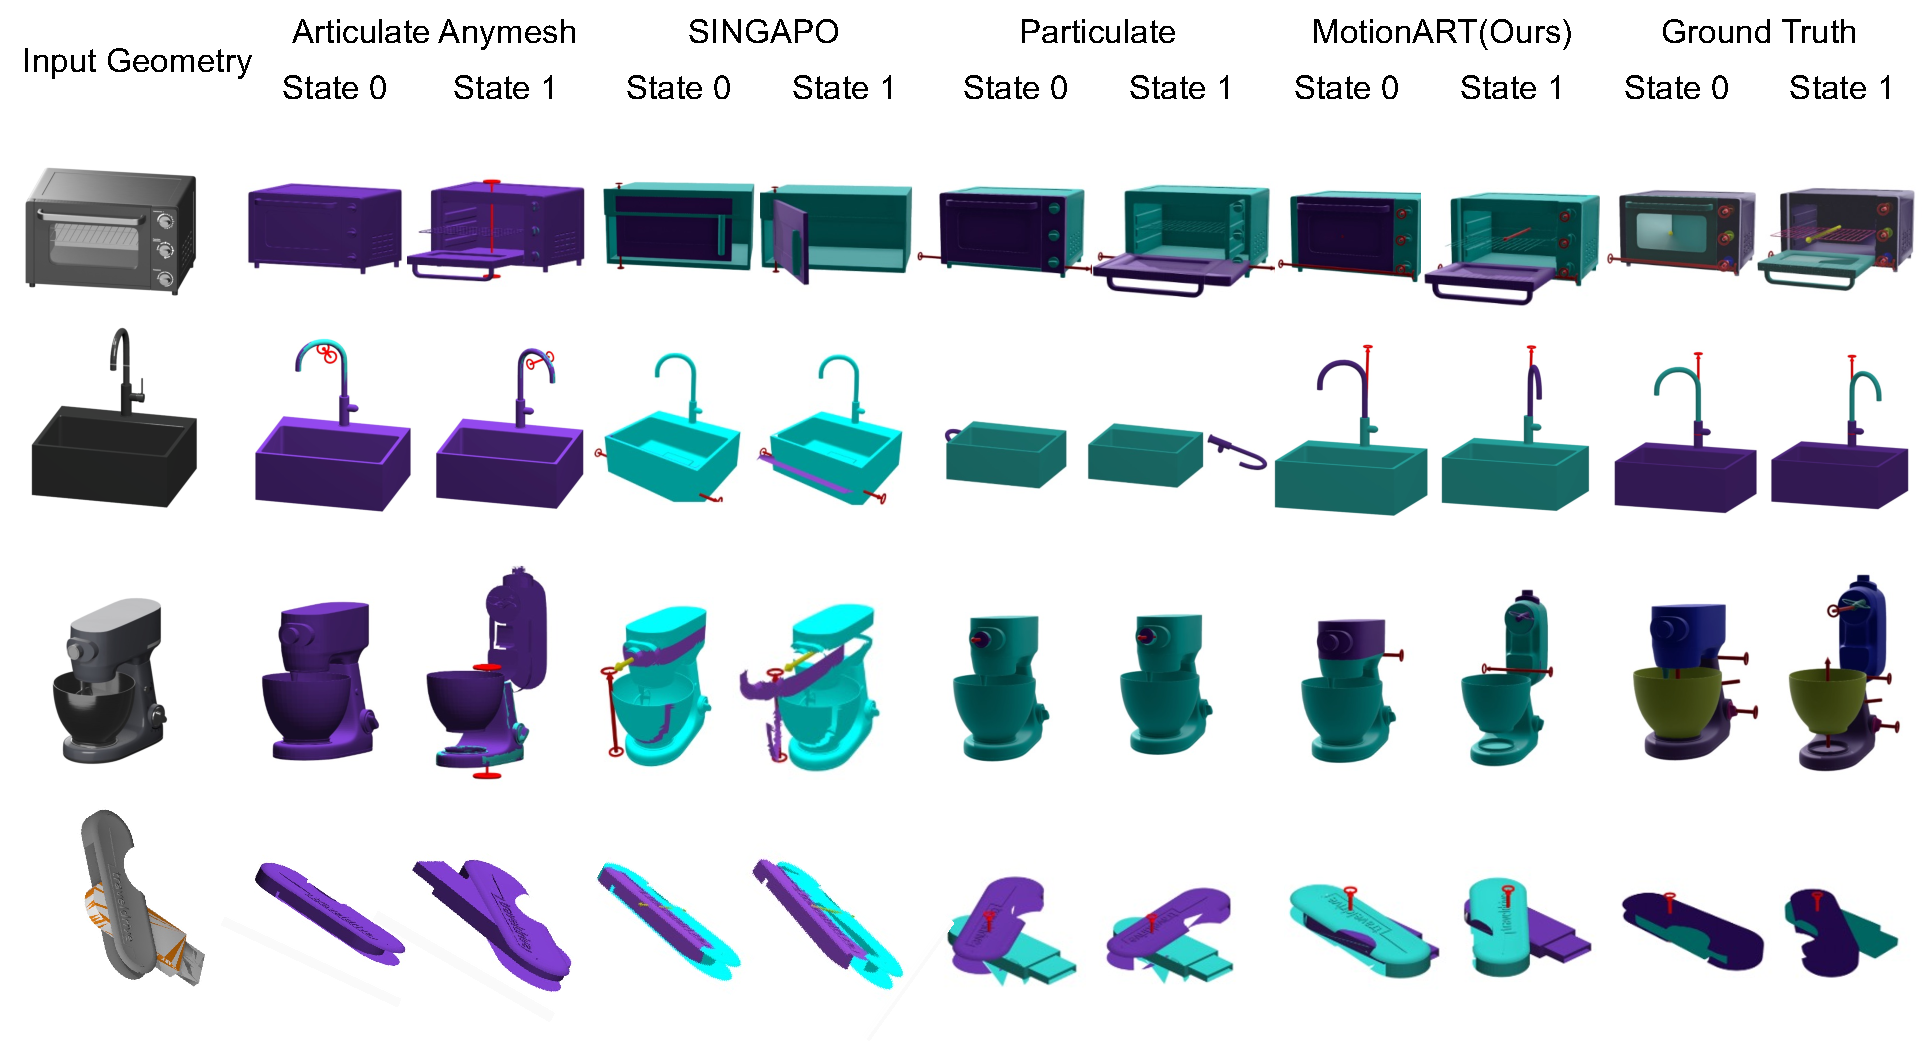
\includegraphics[width=\textwidth]{figs/results_compare.pdf}
  \caption{Qualitative comparison of articulation prediction. We visualize the articulated object in both the rest and fully articulated states. Given the same object, \method predicts more precise part segmentation and better articulation motion on both states than the state-of-the-art methods.}
  \label{fig:qualitative_results}
\end{figure}

% \begin{table}[t]
\centering
\small
\caption{
\textbf{Evaluation on the rest and fully articulated states.}
% For the fully articulated states, every part is moved to its maximum extent. 
We report generalized IoU (gIoU) and part-wise Chamfer distance (PC) for both states. Additionally, we report mean IoU (mIoU) for the rest of the states (computed with penalties for unmatched parts) and whole-object Chamfer distance (OC) for the fully articulated states (measuring the overall bidirectional Chamfer distance between the \emph{whole} predicted geometry and its GT counterpart).
--: SINGAPO assumes mesh connectivity between parts and is not applicable to the PartNet-Mobility test set.
1@10: computed using the best sample out of 10 predictions per instance.
Colors: \best{best} and \secondbest{second best}.
}%
\label{tab:combined-comparison}
% \vspace{-1em}
\setlength{\tabcolsep}{3pt}
\renewcommand{\arraystretch}{1.05}
% 引入 array 宏包并在导言区定义等宽的居中列，例如:
% \usepackage{array}
% \newcolumntype{C}{>{\centering\arraybackslash}p{1.9cm}}
% \resizebox{\linewidth}{!}{%
\begin{tabular}{@{}l *{6}{>{\centering\arraybackslash}p{1cm}} @{}}
\toprule
 & \multicolumn{3}{c}{\textbf{Lightwheel}} & \multicolumn{3}{c}{\textbf{PartNet-Mobility}} \\
\cmidrule(lr){2-4}\cmidrule(lr){5-7}
\textbf{Method}
& gIoU$\uparrow$
& PC$\downarrow$
& $\Delta$
& gIoU$\uparrow$
& PC$\downarrow$
& $\Delta$ \\
\midrule
\multicolumn{7}{c}{\textbf{(a) Rest States ($\Delta$: mIoU$\uparrow$)}} \\
\midrule
PartField~\cite{liu2025partfield} & 0.079 & \best{0.106} & 0.264  & 0.183 & 0.123 & 0.361 \\
P3SAM~\cite{ma2025p3sam}    & 0.122 & 0.177 & 0.411 & -0.116 & 0.261 & 0.267 \\
SINGAPO~\cite{liusingapo}   & -0.097 & 0.234 & 0.273 & 0.262 & 0.124 & 0.468 \\
SINGAPO~\cite{liusingapo} (1@10)  & -0.050 & 0.221 & 0.297 &   0.271 & 0.117 & 0.471 \\
Articulate AnyMesh~\cite{qiu2025articulate}   & 0.172 & 0.190 & 0.452 & 0.383 & 0.104 & 0.542 \\
Particulate~\cite{li2025particulate} & \secondbest{0.332} & {0.168} & \secondbest{0.576} & \secondbest{0.880} & \secondbest{0.003} & \secondbest{0.884}\\
ours          & \best{0.544} & \secondbest{0.156} & \best{0.647} & \best{0.924} & \best{0.002} & \best{0.936} \\
\midrule
\multicolumn{7}{c}{\textbf{(b) Fully Articulated States ($\Delta$: OC$\downarrow$)}} \\
\midrule
SINGAPO~\cite{liusingapo}    & -0.102 & 0.329 & 0.018 &  0.255 & 0.184 & 0.046 \\
SINGAPO~\cite{liusingapo} (1@10)    & -0.056 & 0.261 & 0.019 &  0.264 & 0.168 & 0.041 \\
Articulate AnyMesh~\cite{qiu2025articulate}   & 0.158 & 0.237 & 0.010 & 0.378 & 0.251 & 0.022 \\
Particulate~\cite{li2025particulate}    & \secondbest{0.305} & \secondbest{0.208} & \secondbest{0.009} & \secondbest{0.843} & \secondbest{0.022} & \secondbest{0.003} \\
ours            & \best{0.512} & \best{0.188} & \best{0.005} & \best{0.888} & \best{0.007} & \best{0.001}\\
\bottomrule
\end{tabular}%
% } %
\end{table}
% 
\begin{table}[t]
\centering
\small
\caption{
\textbf{Evaluation on the rest states.}
We report generalized IoU (gIoU), part-wise Chamfer distance (PC), and mean IoU (mIoU), all computed with penalties applied to unmatched parts.
% $^\dagger$: leveraging mesh connectivity.
--: SINGAPO assumes mesh connectivity between parts and is not applicable to the PartNet-Mobility test set.
1@10: computed using the best sample out of 10 predictions per instance.
Colors: \best{best} and \secondbest{second best}.
}%
\label{tab:rest-comparison}
\vspace{-1em}
\setlength{\tabcolsep}{3pt}
\renewcommand{\arraystretch}{1.05}
% \resizebox{\linewidth}{!}{%
\begin{tabular}{@{}lcccccc@{}}
\toprule
 & \multicolumn{3}{c}{\textbf{Lightwheel}} & \multicolumn{3}{c}{\textbf{PartNet-Mobility}} \\
\cmidrule(lr){2-4}\cmidrule(lr){5-7}
%
\textbf{Method}
& gIoU$\uparrow$
& PC$\downarrow$
& mIoU$\uparrow$
& gIoU$\uparrow$
& PC$\downarrow$
& mIoU$\uparrow$ \\
%
% \midrule
%
% Naive Baseline & 0.018 & 0.285 & 0.413 & 0.296 & 0.210 & 0.612 \\
% SINGAPO~\cite{liusingapo}        & -0.116 & 0.201 & 0.272 & -- & -- & -- \\
% SINGAPO~\cite{liusingapo} (1@10)        & -0.096 & 0.190 & 0.277 & -- & -- & -- \\

\midrule
PartField~\cite{liu2025partfield} & 0.079 & \best{0.106} & 0.264  & 0.183 & 0.123 & 0.361 \\
P3SAM~\cite{ma2025p3sam}    & 0.122 & 0.177 & 0.411 & -0.116 & 0.261 & 0.267 \\
SINGAPO~\cite{liusingapo}   & -0.097 & 0.234 & 0.273 & 0.262 & 0.124 & 0.468 \\
SINGAPO~\cite{liusingapo} (1@10)  & -0.050 & 0.221 & 0.297 &   0.271 & 0.117 & 0.471 \\
Articulate AnyMesh~\cite{qiu2025articulate}   & 0.172 & 0.190 & 0.452 & 0.383 & 0.104 & 0.542 \\
Particulate~\cite{li2025particulate} & \best{0.332} & \secondbest{0.168} & \best{0.576} & \secondbest{0.880} & \secondbest{0.003} & \secondbest{0.884}\\


ours (single query)          & {0.489} & {0.163} & {0.578} & \best{0.924} & \best{0.002} & \best{0.936} \\
\bottomrule
\end{tabular}%
% } %
\end{table}



\heading{Articulated-state reconstruction}
\Cref{tab:combined-comparison} (\textbf{Articulated State}) evaluates whether the recovered articulation remains correct after applying the predicted motion.
\method achieves the best performance across all articulated-state metrics, including whole-object Chamfer distance (reducing it from 0.09 to 0.03, a 66\% improvement).
Because this evaluation actuates each predicted joint to its maximum extent, the result validates more than static segmentation: the predicted kinematic structure, motion type, axis, and range must be mutually consistent.
The gap between rest-state and articulated-state performance also reveals why the evaluation should include motion-based metrics; a method can segment parts reasonably while still producing an incorrect joint that fails after actuation.
\Cref{fig:qualitative_results} visualizes representative predictions across object categories.
All state-of-the-art methods struggle with the ``switch'' on ``microwave'',
the ``arm'' of the ``Mixer''.
\method better captures the motion of these small, protruding parts, which are often visually ambiguous in the rest state but become more distinguishable when observing how they move.
This supports the quantitative trend: observing how geometry changes gives the model a more reliable cue for separating functional parts and predicting their motion.

% 
\begin{table}[t]
\centering
\small
\caption{
\textbf{Evaluation on the fully articulated states}, where every part is moved to its maximum extent.
We report part-wise gIoU and PC as in \Cref{tab:rest-comparison}, and whole-object Chamfer distance (OC), which measures the overall bidirectional Chamfer distance between the \emph{whole} predicted geometry and its GT counterpart.
Notations --, 1@10: same as \Cref{tab:rest-comparison}.
Colors: \best{best} and \secondbest{second best}.
}
\vspace{-1em}
\label{tab:full-comparison}
\setlength{\tabcolsep}{3pt}
\renewcommand{\arraystretch}{1.05}
% \resizebox{\linewidth}{!}{%
\begin{tabular}{@{}lcccccc@{}}
\toprule
 & \multicolumn{3}{c}{\textbf{Lightwheel}} & \multicolumn{3}{c}{\textbf{PartNet-Mobility}} \\
\cmidrule(lr){2-4}\cmidrule(lr){5-7}
%
\textbf{Method} & gIoU$\uparrow$ & PC$\downarrow$ & OC$\downarrow$
& gIoU$\uparrow$ & PC$\downarrow$ & OC$\downarrow$ \\

% \midrule
% Naive Baseline & 0.016 & 0.293 & 0.017 & 0.296 & 0.216 & 0.027 \\
% SINGAPO~\cite{liusingapo}     & -0.121 & 0.299 & 0.011 & -- & -- & -- \\
% SINGAPO~\cite{liusingapo} (1@10)  & -0.100 & 0.238 & 0.012 & -- & -- & -- \\

\midrule
SINGAPO~\cite{liusingapo}    & -0.102 & 0.329 & 0.018 &  0.255 & 0.184 & 0.046 \\
SINGAPO~\cite{liusingapo} (1@10)    & -0.056 & 0.261 & 0.019 &  0.264 & 0.168 & 0.041 \\
Articulate AnyMesh~\cite{qiu2025articulate}   & 0.158 & 0.237 & 0.010 & 0.378 & 0.251 & 0.022 \\
Particulate~\cite{li2025particulate}    & \best{0.305} & \best{0.208} & \secondbest{0.009} & \secondbest{0.843} & \secondbest{0.022} & \secondbest{0.003} \\
ours (single query)           & {0.474} & {0.194} & \best{0.003} & \best{0.888} & \best{0.007} & \best{0.001}\\
\bottomrule
\end{tabular}%
% }
\end{table}

\begin{table}[tb!]
    \centering
    \caption{\textbf{Ablation study on model design choices.}
    % We evaluate the contribution of different input-state configurations and training objectives. 
    % In the single-branch setting, we compare models using different numbers of observed states and further ablate the attention mask. 
    % In the Siamese setting, we study the effect of the cycle-consistency loss and compare it with the final model. 
    The ablation is done using a subset of training and evaluation data.
    We report reconstruction quality on both the rest and articulated states, together with inference time. 
    Best results are highlighted in \textbf{bold}.}
    \label{tab:ablation}
    \renewcommand{\arraystretch}{1.0}

    \begin{tabular}{@{} l ccc ccc c @{}}
        \toprule
        \multirow{2}{*}{\textbf{Method}} 
        & \multicolumn{3}{c}{\textbf{Rest state}} 
        & \multicolumn{3}{c}{\textbf{Articulated state}} 
        & \multirow{2}{*}{\textbf{Time}} \\
        \cmidrule(lr){2-4} \cmidrule(lr){5-7}
        & gIoU$\uparrow$ & PC$\downarrow$ & mIoU$\uparrow$ 
        & gIoU$\uparrow$ & PC$\downarrow$ & OC$\downarrow$ 
        & \\
        \midrule

        \multicolumn{8}{l}{\underline{\textbf{Single branch}}} \\
        \textbf{1-state}     
        & {0.305} & {0.096} & {0.480} & {0.293} & {0.144} & {0.008} & {7s} \\
        
        \textbf{2-state (default)}    
        & {0.396} & {0.083} & {0.531} & {0.382} & {0.127} & \textbf{0.004} & {10s} \\
        
        \textbf{4-state}     
        & {0.440} & {0.074} & {0.565} & {0.424} & {0.092} & \textbf{0.004} & {15s} \\
        
        \textbf{8-state}     
        & {0.456} & \textbf{0.073} & {0.574} & \textbf{0.447} & \textbf{0.088} & \textbf{0.004} & {18s} \\
        
        \textbf{w/o attn. mask}  
        & {0.386} & {0.093} & {0.540} & {0.371} & {0.134} & {0.007} & {10s} \\ 

        \midrule 
        \multicolumn{8}{l}{\underline{\textbf{Siamese}}} \\
        
        \textbf{w/o cycle loss} 
        & {0.419} & {0.085} & {0.560} & {0.403} & {0.127} & {0.005} & {10s} \\

        \textbf{final model} 
        & \textbf{0.462} & {0.074} & \textbf{0.578} & {0.445} & {0.112} & \textbf{0.004} & {10s} \\        
        
        \bottomrule
    \end{tabular}
\end{table}


% \heading{Qualitative results}


\subsection{Ablation Study}
\label{sec:exp_ablations}

We conduct thorough ablations to understand the contribution of different design choices in \method.
Results are summarized in \Cref{tab:ablation} and discussed in detail below.

\heading{Importance of Motion States}
Learning from different states serves as a cornerstone of our method,
which formulates articulation recovery as a corresponding motion matching problem.
To measure out motion evidence, we compare the default two-state model with a single-state variant.
When only one state is observed, the quantitative results drop significantly: gIoU drops from 0.396 to 0.305 on the rest state and from 0.382 to 0.293 on the articulated state (nearly 25\% drop), confirming that the second state provides critical evidence for part segmentation and articulation inference.

\heading{Ablations on Number of States}
Our default model uses two states, but the architecture can be flexibly extended to more states.
To verify whether more states can further contribute to performance,
we train a multi-state variant.
The results show that more states do improve performance,
with the 4-state model achieving 0.424 gIoU on the articulated state,
and the 8-state model further improved to 0.447,
but with diminishing returns and increased inference time.

\heading{Ablations on Masked attention}
The attention mask further improves segmentation quality by encouraging part queries to focus on their activated regions across transformer layers.

\heading{Ablations on Siamese Network}
We further demonstrate that the Siamese architecture, along with the cycle-consistency loss, improves the consistency of predictions between the two states.
The Siamese model achieves the best or second-best performance compared with the single-branch models,
even though the single-branch model with 8 states has more input information.
However, removing the cycle-consistency loss from the Siamese model leads to a significant drop in performance, especially for articulated states, indicating that the cycle loss is crucial for stabilizing part identity and motion direction when the state order is reversed.

\begin{figure}[t]
  \centering
  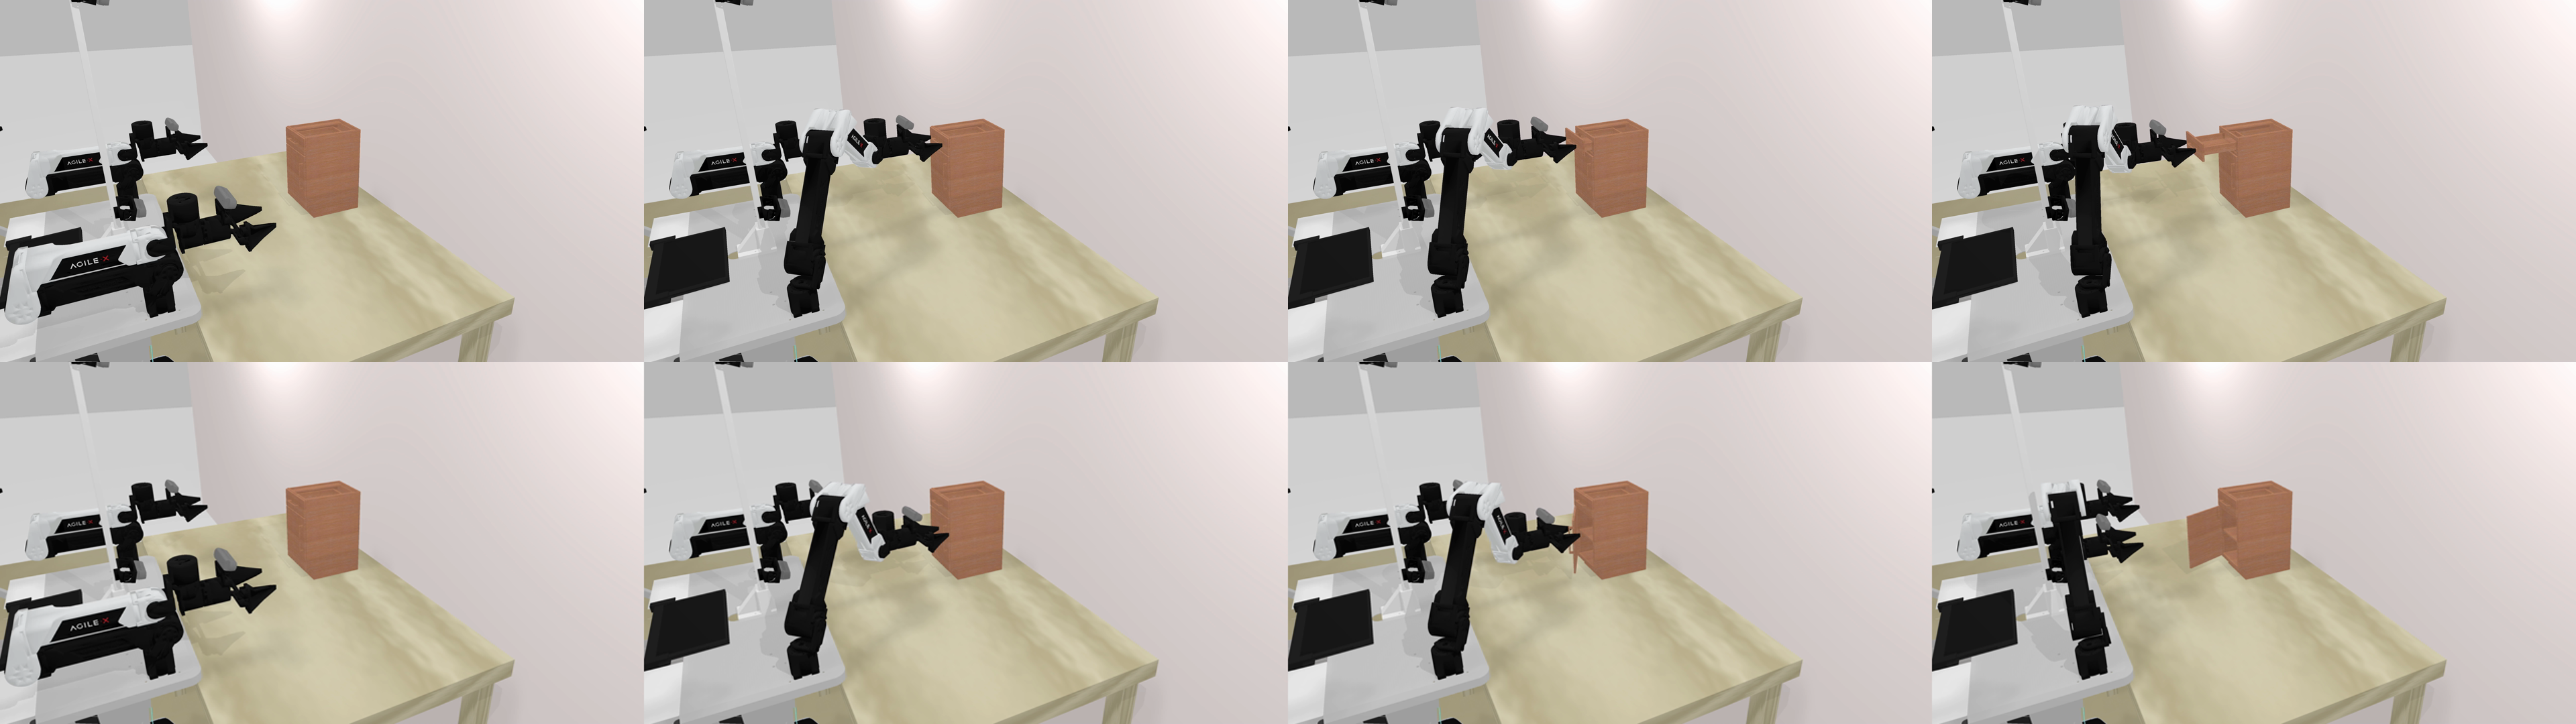
\includegraphics[width=\textwidth]{figs/4_application.png}
  \caption{\textbf{RoboTwin application with generated URDF assets.}
  We export \method{}'s predicted articulated structures as URDF assets and import them into RoboTwin.
  Each row shows four snapshots of contact-based manipulation: a drawer asset (top) and a door asset (bottom) are opened by a robot arm using the predicted movable link, joint axis, and motion range.}
  \label{fig:_application}
\end{figure}


\subsection{Application}
\label{sec:exp_application}

We further test whether the predicted articulation can be exported as a usable robot-simulation asset.
To this end, we convert the outputs to a URDF.
% predicted part masks into link meshes and instantiate the predicted kinematic tree, joint types, axes, and ranges as a URDF.
As shown in~\cref{fig:_application}, the generated drawer and door assets can be loaded into RoboTwin and opened by a robot arm through contact.
% This application checks a property that static reconstruction metrics do not directly measure.
For the robot to open the generated asset, the predicted movable part, joint axis, and motion range must remain mutually consistent under physics-based interaction.
The RoboTwin result, therefore, provides a compact qualitative validation that two-state geometry can support not only offline articulation recovery but also downstream manipulation of generated articulated assets.

\section{Conclusion}%
\label{sec:conclusions}

We presented \method, a feed-forward framework for inferring articulated 3D structure from \emph{two} observed states of the same object.
% The key to our success is that we learn articulation from two states' motion evidence.
It departs from the common feed-forward methods,
which typically learns articulation from a \emph{single} state and relies heavily on category-level priors to infer part motion.
It achieves state-of-the-art performance on both rest-state part segmentation and articulated-state reconstruction, with a single forward pass and no post-processing.
The ablations further validate the importance of motion evidence, siamese paired learning, and cycle-consistency training.
Beyond metrics, we also demonstrate a direct application in which the predicted articulated object is exported as a URDF asset and interacts with a robot arm in the RoboTwin simulator.

% The central idea is that articulation is most directly revealed by state change: two independently sampled point clouds reveal which parts move together and how their motion is constrained, reducing reliance on category-level priors learned from limited annotations.
% To exploit this cue, \method uses shared part queries, cross-state transformer reasoning, mask-guided point-query refinement, and a Siamese cycle-consistency objective to predict part segmentation and articulation parameters in a single-pass pipeline.
% All the proposed designs are further proven valid in the experiments.
% % Experiments show that the two-state formulation improves both rest-state part recovery and articulated-state reconstruction, while ablations validate the role of cross-state input, attention masking, and cycle-consistency training.
% Beyond metrics, we also demonstrate a direct application in which the predicted articulated object is exported as a URDF asset and interacts with a robot arm in the RoboTwin simulator.
% This result suggests that multi-state geometry can serve as a practical bridge between visual or generated object observations and simulation-ready articulated assets for downstream embodied interaction.

% Several limitations remain.

% Future work can extend this formulation to noisy image-derived reconstructions, richer joint constraints, multi-step state sequences, and closed-loop robot interaction, where the agent actively chooses actions that reveal the most informative articulation evidence.


\subsection*{AI use statement}

\textbf{TODO before submission:} Replace this placeholder with the authors'
ICLR 2027 AI use disclosure. Describe every required or recommended use of
generative AI, how the outputs were checked, and the authors' responsibility
for the final paper, code, claims, and artifacts.

% Add an Ethics Statement here if the work raises relevant concerns.
% Add a Reproducibility Statement here if desired; ICLR strongly recommends it.


\ificlrfinal
\subsubsection*{Acknowledgments}
Acks.
\fi

\bibliography{chuanxia_general,chuanxia_specific,main}
\bibliographystyle{iclr2027_conference}

\appendix
\clearpage

\begin{center}
    {\Large\textbf{What Reveals 3D Articulation? Learning from Motion}}

    \vspace{0.1in}
    % {\Large\textbf{\textit{Supplementary Material}}}
    {{\textit{Supplementary Material}}}

    \vspace{0.1in}
    % Anonymous project page: \url{}

\end{center}

\section{Related Work}
\label{sec:supp_related_work}


We provide a comparison table of related works as shown in~\Cref{tab:related_articulation}.
\begin{table}[ht]
\centering
\small
\setlength{\tabcolsep}{2.5pt} % 稍微收缩列间距，防止表格过宽
\renewcommand{\arraystretch}{1.2} % 增加行高，让表格更有呼吸感
\resizebox{\linewidth}{!}{%
\begin{tabular}{@{}l ccccc | cccccc c | c @{}}
\toprule
& \multicolumn{5}{c|}{\textbf{Input Modality}} & \multicolumn{7}{c|}{\textbf{Output Properties}} & \textbf{Inf.} \\
\cmidrule(lr){2-6} \cmidrule(lr){7-13}
\textbf{Method} & \faAlignLeft & \faCamera & \faProjectDiagram & \textbf{3D} & \faLayerGroup & \faBoxOpen & \textbf{3D} & \faShapes & \faProjectDiagram & \faLongArrowAltRight & \faArrowsAltV & $\mathbf{1}^{+}$ & \textbf{Time} \\
\midrule

% --- 第一类：基于优化的方法 ---
\rowcolor{tableblue} \multicolumn{14}{l}{\textit{Optimization-based Methods}} \\
PARIS \cite{liu2023paris} & -- & \checkmark & -- & -- & 2 & -- & \checkmark & \checkmark & \checkmark & \checkmark & \checkmark & -- & N/A \\
AIM \cite{ai2026aim}& -- & \checkmark & -- & \checkmark & 2 & -- & \checkmark & \checkmark & \checkmark & \checkmark & \checkmark & \checkmark & N/A \\

\midrule
% --- 第二类：基于学习的方法 ---
\rowcolor{tableblue} \multicolumn{14}{l}{\textit{Learning-based Methods}} \\
GEOPARD \cite{Goyal_2025_ICCV} & -- & -- & -- & \checkmark$^\dagger$ & 1 & -- & \checkmark & -- & \checkmark & \checkmark & -- & \checkmark & N/A \\
MeshArt \cite{gao2025meshart} & -- & (\checkmark)$^o$ & -- & (\checkmark)$^o$ & 0 & \checkmark & \checkmark & \checkmark & -- & \checkmark & \checkmark & \checkmark & N/A \\
PARTICULATE \cite{li2025particulate} & -- & -- & -- & \checkmark & 1 & -- & \checkmark & \checkmark & \checkmark & \checkmark & \checkmark & \checkmark & \textasciitilde10s \\
URDF-Anything \cite{li2025urdfanything} & \checkmark & \checkmark & -- & \checkmark & 1 & -- & \checkmark & \checkmark & \checkmark & \checkmark & \checkmark & \checkmark & N/A \\

\midrule
% --- 第三类：基于检索的方法 ---
\rowcolor{tableblue} \multicolumn{14}{l}{\textit{Generation-based Methods}} \\
SINGAPO \cite{liusingapo} & -- & \checkmark & -- & -- & 1 & \checkmark & (\checkmark)$^\ast$ & \checkmark & \checkmark & \checkmark & \checkmark & \checkmark & \textasciitilde10s \\
CAGE \cite{liu2024cage} & \checkmark & -- & \checkmark & -- & 1 & \checkmark & (\checkmark)$^\ast$ & \checkmark & \checkmark & \checkmark & -- & \checkmark & N/A \\
Kinematify \cite{wang2025kinematify} & (\checkmark)$^o$ & (\checkmark)$^o$ & -- & -- & (1)$^o$ & -- & \checkmark & \checkmark & \checkmark & \checkmark & -- & \checkmark & \textasciitilde20m \\
Articulate-Anything \cite{le2024articulate} & \checkmark & (\checkmark)$^o$ & -- & -- & (1$^{+}$)$^o$ & -- & (\checkmark)$^\ast$ & \checkmark & \checkmark & \checkmark & \checkmark & -- & \textasciitilde10m \\
FreeArt3D \cite{chen2025freeart3d} & -- & \checkmark & \checkmark & -- & 6 & -- & \checkmark & \checkmark & \checkmark & \checkmark & -- & -- & \textasciitilde10m \\
Articulate AnyMesh \cite{qiu2025articulate} & -- & -- & -- & \checkmark & 1 & -- & \checkmark & \checkmark & \checkmark & \checkmark & \checkmark & \checkmark & N/A \\
DreamArt \cite{lu2025dreamart} & -- & \checkmark & -- & -- & 1 & -- & \checkmark & \checkmark & -- & \checkmark & \checkmark & -- & N/A \\
URDF-Anything+ \cite{wu2026urdfanything_plus}& -- & \checkmark & -- & \checkmark & 1 & -- & \checkmark & \checkmark & \checkmark & \checkmark & \checkmark & \checkmark & N/A  \\ 
ArtiLatent \cite{chen2025ArtiLatent} & -- & (\checkmark)$^o$ & -- & -- & (1)$^o$ & -- & \checkmark & \checkmark & \checkmark & \checkmark & \checkmark & \checkmark & \textasciitilde30s \\
ArtFormer \cite{Su_2025_CVPR} & \checkmark & (\checkmark)$^o$ & -- & -- & (1)$^o$ & \checkmark & \checkmark & \checkmark & \checkmark & \checkmark & \checkmark & \checkmark & N/A \\


\midrule
% --- 你的方法 ---
\rowcolor{blue!15} \textbf{Ours} & -- & -- & -- & \checkmark & 2 & -- & \checkmark & \checkmark & \checkmark & \checkmark & \checkmark & \checkmark & \best{\textasciitilde10s} \\
\bottomrule
\end{tabular}%
}
\caption{
\textbf{Related work overview on articulated object modeling.} 
We summarize input modalities, the number of observed articulation configurations, and output properties for various methods. 
Icons represent: 
\faAlignLeft\ Text, 
\faCamera\ Vision(e.g., image or video), 
\faProjectDiagram\ Kinematic Chain, 
\textbf{3D} Geometry(e.g., mesh or point cloud), 
\faLayerGroup\ Number of observed articulation configurations. 
State counts are modality-agnostic: image, video, mesh, and point-cloud observations are counted by articulation configuration.
0 denotes generation without an observed object state; $(\cdot)^o$ denotes optional conditioning, e.g., $(1)^o$ for one optional state and $(1^+)^o$ for one or more optional states.
Output columns show: 
\faBoxOpen\ BBox, 
\textbf{3D} Geometry(e.g., mesh or point cloud), 
\faShapes\ Segmentation, 
\faProjectDiagram\ Structure, 
\faLongArrowAltRight\ Axis, 
\faArrowsAltV\ Range, 
$\mathbf{1}^{+}$ Multi-joint support.
($^\ast$) denotes retrieval-based geometry. 
($^o$) indicates optional conditional inputs or outputs. 
($^\dagger$) requires pre-segmented geometry.
N/A indicates the inference time is not reported in the original paper.
}
\label{tab:related_articulation}
\end{table}


\section{Implementation Details}
\label{sec:supp_details}

\subsection{Data Processing}
\label{sec:supp_data_processing}

We preprocess articulated assets from URDF and USD sources into a unified representation for two-state articulation learning. The pipeline first converts articulated objects into normalized meshes with part-level motion annotations, then samples point clouds from the exported meshes to cache training supervision.

\paragraph{URDF processing.}
For URDF assets, we parse each object's kinematic tree and mesh references, then export two canonical articulation states. Each processed object is written to an object-level directory, where \texttt{pos\_000} corresponds to the all-zero joint state and \texttt{pos\_001} corresponds to the all-one joint state. For each state, the links are transformed by forward kinematics and merged into a single mesh. We filter out invalid assets that contain no valid mesh, only one articulated part, or more than the maximum allowed number of parts. In our preprocessing, we set this maximum to 16.
% 
To keep the two states geometrically comparable, we compute a shared normalization transform over all exported states of the same object and apply it consistently to every posed mesh. The same normalization is applied to motion annotations: prismatic ranges are scaled, and revolute or prismatic axes are shifted into the normalized coordinate frame.

\paragraph{USD processing.}
For USD assets, we follow the same output convention while extracting articulation information from USD physics joints. We traverse the USD stage, identify revolute, prismatic, and fixed joints, recover parent-child link relationships, and compute each joint axis and anchor in world coordinates. We then solve forward kinematics for the two articulation states, export each posed mesh, and save the same metadata files as in the URDF pipeline.
% 
The USD pipeline also normalizes all generated states of an object jointly. After all posed meshes are exported, we compute a shared object-level center and scale, rewrite the normalized OBJ files, and transform the saved Plucker axes and motion ranges accordingly. 

\paragraph{Point sampling and cached supervision.}
After mesh export, we cache point-level supervision from each normalized mesh. For each mesh, we sample surface points with their normals and assign them to the articulated parts using the vertex-to-part labels. To better preserve geometric discontinuities between parts, training samples combine uniformly sampled surface points with points sampled near sharp edges. If no sharp edges are detected, the sampler falls back to uniform surface sampling.
% 
For training, each cached point cloud stores the sampled point cloud, normals, point-to-part labels, a binary indicator for sharp-edge samples, the part hierarchy, and per-part motion annotations.
% 
This cached representation removes the need to repeatedly load articulated meshes during training and provides a unified supervision format across URDF- and USD-derived objects.

\subsection{Training Loss Details}
\label{sec:supp_loss_details}

For cycle consistency, we enforce that the Siamese branch produces symmetric predictions. Given the reserve-order states as input, we hope the network produces part segmentation results that are consistent with those of the forward-order branch, but with opposite articulation motion. Therefore, we first swap the order of part segmentation results in the reverse branch from $\{\hat{M}_{r}^{(s_1)},\hat{M}_{r}^{(s_0)}\}$ to $\{\hat{M}_{r}^{(s_0)},\hat{M}_{r}^{(s_1)}\}$, matching the corresponding segmentation masks in forward branch.
Then we maintain the axis of articulation motion and flip the predicted revolute range and prismatic range from $\alpha_r = \{\alpha_{\min}, \alpha_{\max}\}, l_r = \{l_{\min}, l_{\max}\}$ to $\dot{\alpha}_r = \{\alpha_{\max}, \alpha_{\min}\}, \dot{l}_r = \{l_{\max}, l_{\min}\}$, representing opposite motion.
In this way, the model faithfully learns the underlying physical laws hidden in state changes.


\section{Additional Experimental Results}
\label{sec:supp_additional_experiments}

\paragraph{Additional Ablations.}
We provide additional ablation results under two evaluation protocols.
The no-penalty protocol reports part-wise metrics after matching predicted and ground-truth parts without penalizing unmatched parts, while the penalty protocol assigns penalties to unmatched predictions or missing ground-truth parts.
Reporting both protocols helps separate two effects: how well a model aligns the parts it finds and whether it recovers all functional parts required for a complete articulated asset.

\begin{table}[!htbp]
    \centering
    \caption{\textbf{Additional ablation results without unmatched-part penalty.}
    We use the same ablation variants and metrics as in the main ablation table, but compute the part-wise metrics without penalizing unmatched predicted or ground-truth parts.}
    \label{tab:supp-ablation-without-penalty}
    \renewcommand{\arraystretch}{1.2}

    \begin{tabular*}{\linewidth}{@{\extracolsep{\fill}} l ccc ccc c @{}}
        \toprule
        \multirow{2}{*}{\textbf{Method}}
        & \multicolumn{3}{c}{\textbf{Rest state}}
        & \multicolumn{3}{c}{\textbf{Articulated state}}
        & \multirow{2}{*}{\textbf{Inf. Time}} \\
        \cmidrule(lr){2-4} \cmidrule(lr){5-7}
        & gIoU$\uparrow$ & PC$\downarrow$ & mIoU$\uparrow$
        & gIoU$\uparrow$ & PC$\downarrow$ & OC$\downarrow$
        & \\
        \midrule

        \multicolumn{8}{l}{\underline{\textbf{Single branch}}} \\
        \textbf{1-state}
        & 0.470 & 0.028 & 0.536 & 0.457 & 0.087 & 0.008 & 7s \\

        \textbf{2-state}
        & 0.545 & 0.023 & 0.580 & 0.530 & 0.077 & 0.004 & 10s \\
        
        \textbf{4-state}
        & {0.576} & {0.020} & {0.611} & {0.560} & {0.041} & {0.004} & {15s} \\

        \textbf{8-state}     
        & {0.577} & {0.019} & {0.627} & {0.598} & {0.039} & {0.004} & {18s} \\

        \textbf{w/o attn. mask}
        & 0.567 & 0.024 & 0.602 & 0.561 & 0.084 & 0.007 & 10s \\

        \midrule
        \multicolumn{8}{l}{\underline{\textbf{Siamese}}} \\

        \textbf{w/o cycle loss}
        & 0.583 & 0.020 & 0.619 & 0.567 & 0.074 & 0.005 & 10s \\

        \textbf{final model}
        & 0.578 & 0.027 & 0.617 & 0.560 & 0.075 & 0.004 & 10s \\

        \bottomrule
    \end{tabular*}
\end{table}

\begin{table}[!htbp]
    \centering
    \caption{\textbf{Additional ablation results with unmatched-part penalty.}
    This table follows the main ablation protocol, where unmatched predicted or ground-truth parts are penalized in the part-wise metrics.
    The values are copied from the main ablation table for easier side-by-side comparison with \cref{tab:supp-ablation-without-penalty}.}
    \label{tab:supp-ablation-with-penalty}
    \renewcommand{\arraystretch}{1.2}

    \begin{tabular*}{\linewidth}{@{\extracolsep{\fill}} l ccc ccc c @{}}
        \toprule
        \multirow{2}{*}{\textbf{Method}}
        & \multicolumn{3}{c}{\textbf{Rest state}}
        & \multicolumn{3}{c}{\textbf{Articulated state}}
        & \multirow{2}{*}{\textbf{Inf. Time}} \\
        \cmidrule(lr){2-4} \cmidrule(lr){5-7}
        & gIoU$\uparrow$ & PC$\downarrow$ & mIoU$\uparrow$
        & gIoU$\uparrow$ & PC$\downarrow$ & OC$\downarrow$
        & \\
        \midrule

        \multicolumn{8}{l}{\underline{\textbf{Single branch}}} \\
        \textbf{1-state}
        & {0.305} & {0.096} & {0.480} & {0.293} & {0.144} & {0.008} & {7s} \\

        \textbf{2-state}
        & {0.396} & {0.083} & {0.531} & {0.382} & {0.127} & {0.004} & {10s} \\

        \textbf{4-state}
        & {0.440} & {0.074} & {0.565} & {0.424} & {0.092} & {0.004} & {15s} \\

        \textbf{8-state}     
        & {0.456} & {0.073} & {0.574} & {0.447} & {0.088} & {0.004} & {18s} \\
        \textbf{w/o attn. mask}
        & {0.386} & {0.093} & {0.540} & {0.371} & {0.134} & {0.007} & {10s} \\ 

        \midrule
        \multicolumn{8}{l}{\underline{\textbf{Siamese}}} \\

        \textbf{w/o cycle loss}
        & {0.419} & {0.085} & {0.560} & {0.403} & {0.127} & {0.005} & {10s} \\

        \textbf{final model}
        & {0.462} & {0.074} & {0.578} & {0.445} & {0.112} & {0.004} & {10s} \\

        \bottomrule
    \end{tabular*}
\end{table}


\paragraph{Additional Visualizations.}

We provide additional visualizations in~\Cref{fig:supp_results} and in the video attached to the supplementary folder.

\subsection{Failure Case Analysis}
\label{sec:supp_failure_case}

\begin{figure}[t]
  \centering
  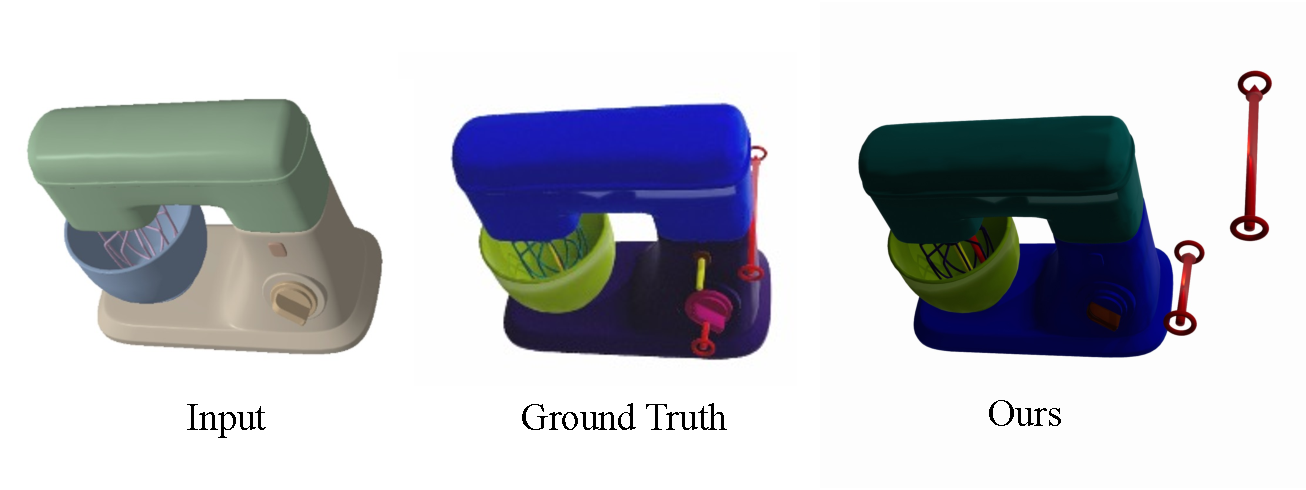
\includegraphics[width=\textwidth]{figs/failure_case.pdf}
  \caption{We show one failure case on a hierarchical object with multiple coupled rotation axes.}
  \label{fig:failure_case}
\end{figure}

\begin{figure}[t]
  \centering
  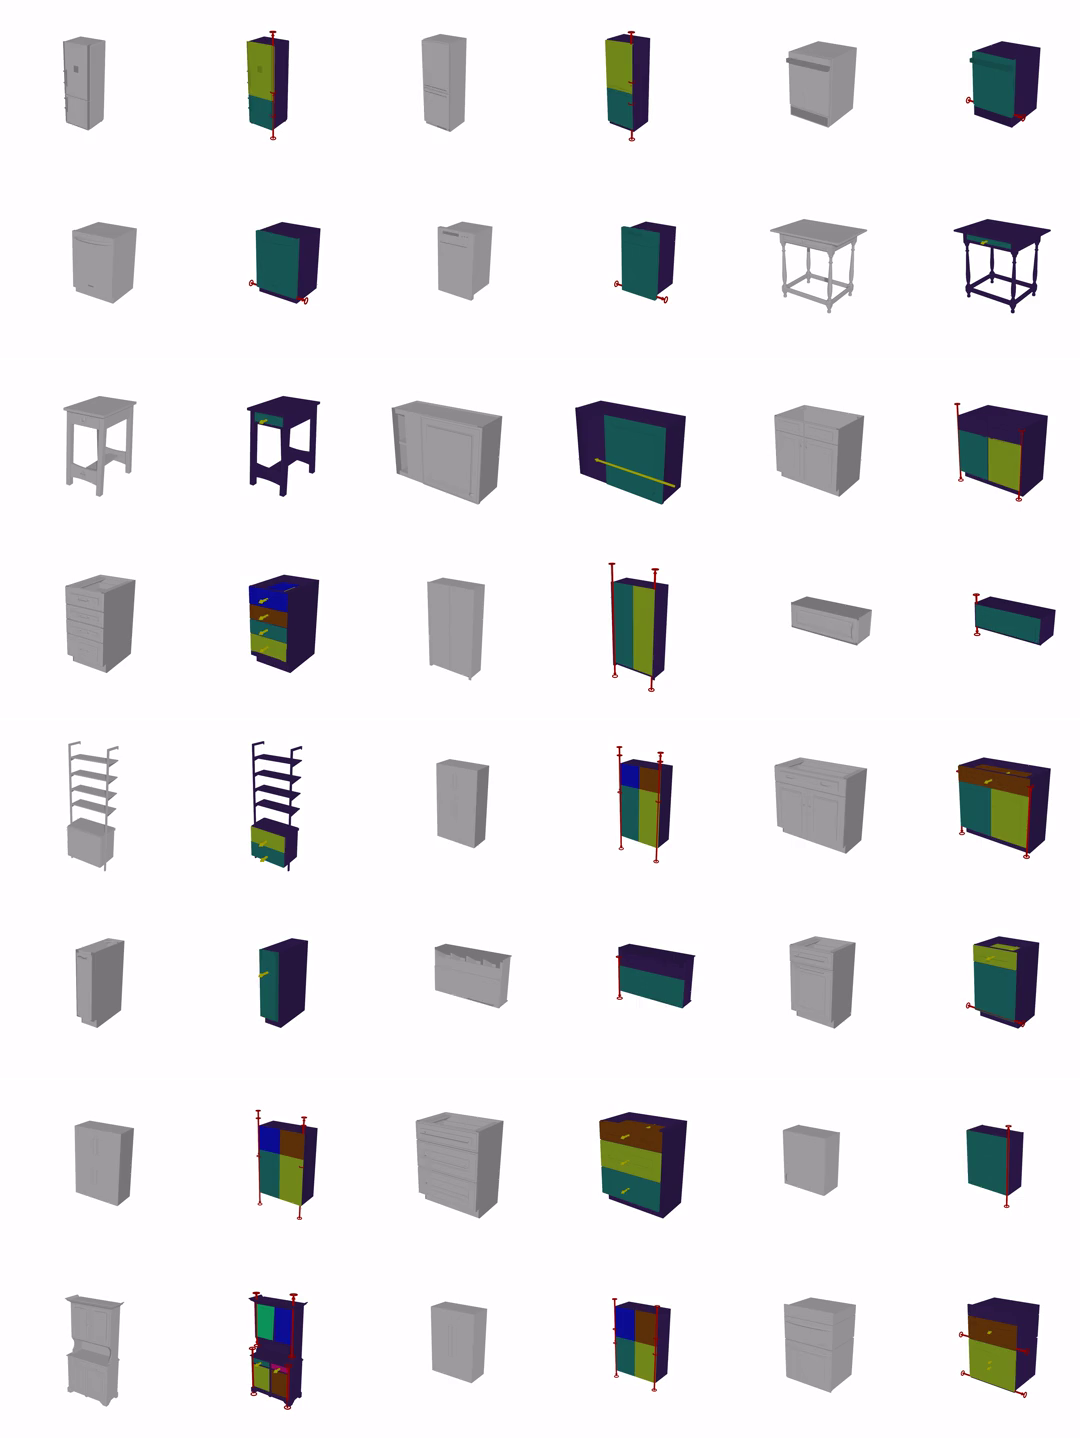
\includegraphics[width=\textwidth]{figs/supp_results.png}
  \caption{We show more visualization examples on the test set of PartNet-Mobility. Plus, we provide a video version to vividly demonstrate the articulation motion.}
  \label{fig:supp_results}
\end{figure}


A representative failure mode of \method occurs on hierarchical objects with multiple coupled rotation axes, as shown in~\Cref{fig:failure_case}.
In these cases, the motion of a child part cannot be explained by an independent joint in a fixed global frame: the child joint axis is itself transformed by the motion of its parent link.
When the parent joint rotates, the coordinate frame in which the child joint is defined also rotates, so the observed displacement of the child part is a composition of the parent motion and the child's own local articulation.
Such configurations are relatively rare in our current training data, making it difficult for a feed-forward model to learn a reliable prior for this form of nested kinematic dependency.

This failure mode is also sensitive to error accumulation along the predicted kinematic tree.
If the parent edge is assigned an inaccurate motion type, axis, pivot, or range, the resulting parent transform changes the reference frame used to interpret all descendant joints.
The child prediction must then compensate for both its own articulation error and the residual error inherited from the parent, which can produce substantially larger deviations after forward kinematic actuation than the per-joint prediction error would suggest.
Therefore, although two-state geometry provides strong evidence for ordinary articulated motion, deeply coupled multi-axis structures remain challenging when the training distribution contains few comparable examples and when small upstream errors propagate to downstream parts.

\section{Limitations.}
Our current formulation assumes that the two observations depict the same object under compatible states and that the target articulation can be represented by a tree-structured URDF.
The method may struggle when the two states differ due to severe reconstruction artifacts, non-rigid deformation, missing geometry, or contacts that hide the moving component.

\section{Statistical Reporting and Impact}
\label{sec:supp_impl_compute_impact}

\paragraph{Statistical reporting.}
For all experimental results, we report a single run under the evaluation protocol.
All reported metrics are computed on the same evaluation split for a given benchmark, and ablations change only the stated model component or training objective.

\paragraph{Broader impact.}
\method can help convert observed or generated articulated objects into simulation-ready assets, benefiting robotics, embodied AI, and virtual-environment construction.
At the same time, incorrect articulation predictions can lead to unreliable simulated interactions, especially if generated assets are used for downstream robot policy training without validation.
We therefore view the predicted URDF assets as candidates that should be checked in simulation before deployment on physical robots, and we encourage users to preserve provenance information for generated or converted assets.



\end{document}
